\documentclass[12pt]{amsart}

\RequirePackage[OT1]{fontenc}

\usepackage[foot]{amsaddr}
% \usepackage{biblatex}
\usepackage{natbib}
%\bibliographystyle{apalike}
\usepackage{multirow}
\usepackage{enumitem}

\usepackage{tchdr}
\boldshortcuts

\usepackage{graphicx}
\usepackage{wrapfig}
\usepackage{setspace}
\DeclareGraphicsExtensions{.eps, .ps}
\usepackage{amsmath, amsthm, amsfonts}
% \usepackage[margin=1.5in]{geometry}

\numberwithin{equation}{section}
\theoremstyle{plain}
\newtheorem{theorem}{Theorem}[section]
% \newtheorem{example}{Example}
% \newtheorem{remark}{Remark}
\newtheorem{corollary}[theorem]{Corollary}
\newtheorem{criterion}[theorem]{Criterion}
\newtheorem{definition}[theorem]{Definition}
\newtheorem{exercise}[theorem]{Exercise}
\newtheorem{lemma}[theorem]{Lemma}
\newtheorem{proposition}[theorem]{Proposition}

\setlength{\textwidth}{6.5in}
\setlength{\textheight}{8.5in}
\setlength{\topmargin}{-0.25in}
\setlength{\evensidemargin}{0in}
\setlength{\oddsidemargin}{0in}
%\setlength{\evensidemargin}{.25in}
%\setlength{\oddsidemargin}{.25in}


\usepackage{setspace}
% \onehalfspacing
\doublespacing


\def\pr{\text{pr}}
\def\sgn{\text{sgn}}
\def\I{\bf I}

\begin{document}

\title[Statistical paradoxes in coronavirus case-counts]{Statistical paradoxes in coronavirus case-counts: selection bias, measurement error, and the COVID-19 pandemic} %

\author{Walter Dempsey}
\address{Department of Biostatistics, University of Michigan, Ann Arbor, MI 48109}
% \email{wdem@umich.edu}

\begin{abstract}
  Coronavirus case-count data has influenced government policies and drives most epidemiological forecasts. Limited testing is cited as the key driver behind minimal information on the COVID-19 pandemic. While expanded testing is laudable, measurement error and selection bias are the two greatest problems limiting our understanding of the COVID-19 pandemic; neither can be fully addressed by increased testing capacity. In this paper, we demonstrate their impact on estimation of point prevalence and the effective reproduction number. We show that estimates based on the millions of molecular tests in the US has the same mean square error as a small simple random sample.  To address this, a procedure is presented that combines case-count data and random samples over time to estimate selection propensities based on key covariate information. We then combine these selection propensities with epidemiological forecast models using death-only data to construct a \emph{doubly-robust} estimation method that accounts for both measurement-error and selection bias.  This method is then applied to estimate Indiana's prevalence using case-count, hospitalization, and death data with cumulative demographic information, the United States's only statewide random molecular sample collected from April 25--29th, and Facebook's COVID-19 symptom survey.  We end with a series of recommendations based on the proposed methodology.
\end{abstract}

\maketitle


\section{Introduction}
The World Health Organization has declared the coronavirus disease 2019 (COVID-19) a public health emergency.  \textcolor{red}{As of June 15th, 2021, over 176 million cases have been confirmed worldwide with 33.4 million cases and over 590 thousand confirmed deaths across the United States.} This pandemic
has become the focal point of everyday life; yet the data landscape for understanding COVID-19 remains limited.  Public databases~\citep{JHU_Lancet,NYT} provide incoming county-level information of confirmed cases and deaths.  Statisticians, epidemiologists, economists, and data scientists have used this granular data to forecast COVID-19 case-counts, deaths, and hospitalizations~\citep{Giordano2020,Song2020,Ray2020,2020.IHME,Wang2020.03,JTD36385}.

This paper has two main objectives.  The first objective is to express reservations at the use of case-counts as a proxy for disease prevalence and in estimation of standard epidemiological models for inference and forecasting.  The reason is straightforward: observed case-count data is plagued by selection bias and measurement error. Through a series of calculations, we will demonstrate that the information gained from increasing testing capacity is limited in the presence of selection bias and when testing inaccuracies persist.  In particular, the millions of tests in the US have a small effective sample size when compared to random sampling. These calculations demonstrate the importance of probabilistic sampling designs over time for estimation of point prevalence and effective reproduction number.

Due to monetary and time constraints, however, random testing is either not performed or performed very infrequently.  As of June 2021, Indiana is the only state to conduct statewide random sample testing\footnote{This is the only random sample to collect both seroprevalence and diagnostic testing results. The CDC has conducted several seroprevalence studies. See Section~\ref{section:testinginfo} for further discussion.}, which was collected from April 25--29, 2020~\citep{Yiannoutsos2021}.  Such infrequent random testing is likely to provide insufficient information to help researchers and policy makers better understand the disease trajectory which can change rapidly over time.  Therefore, while random testing may be preferable in theory, in practice governments, researchers, and policy makers continue to use coronavirus case-counts to understand the impact of COVID-19 on the population and make data-informed decisions.

The second objective is to demonstrate how random samples provide necessary \emph{auxiliary information} to address selection bias in coronavirus case-count data.  Random samples provide the necessary covariate information from a representative sample from the population to estimate selection propensities. These propensities can then used in an inverse-probability weighting scheme to construct estimators of disease prevalence that attempt to control for selection bias.  A doubly robust extension allows researchers to combine these estimates with epidemiological forecasts based on compartmental models that are common in the study of infectious diseases~\cite{Hao2020,Song2020,Ray2020,Johndrow2020}.

Note that the proposed approach requires covariate information to be collected on tested individuals.  Unfortunately, many states do not require or report auxiliary covariate information beyond demographics such as gender, age, race, and ethnicity.  To address this, we discuss how the proposal suggests minor changes to current practice that may improve performance over time. While we demonstrate empirical improvements over simple disease prevalence estimates, we also highlight how selection bias may persist and impact uncertainty quantification.

% Hospitalization Gelman

\subsection{Related work}

This article discusses the relationship between three statistical concepts: selection bias, measurement error, and population size.  We build on the work of \cite{Meng2018} who studied an error decomposition to understand the relationship between selection bias and population size.  In particular, we quantify the interaction between measurement-error and selection bias.  The sign and magnitude of the statistical decomposition can change drastically; the impact on the effective sample size can therefore be quite large.

After demonstrating the limitations of case-count analysis when compared to random sampling, we then assess whether their is potential for combining the \emph{nonprobability samples} with \emph{probability samples} to improve point prevalence estimation. For any probability sampling design, the Horvitz-Thompson estimator~\citep{HT1952} incorporates design information via inverse-probability weights (IPW).  For nonprobability samples, the IPW estimator requires modelling the propensity scores.  Its use in the survey context is also referred to as the quasi-randomization approach~\citep{Elliott2017}. \cite{Valliant2011} consider a weighted logistic regression procedure using the pooled probability and nonprobability samples.  \cite{Chen2019} consider a pseudo-log-likelihood approach that uses the random samples as a proxy for a term in the log-likelihood.  Here, we extend this approach to account for measurement-error as well as random sampling at multiple times. We then provide an extension of the statistical error decomposition and discuss the trade-offs inherent in such a weighting approach.

One core component of coronavirus research is epidemiological state-space modelling of case-count and death data. These models can be used to answer a variety of research questions including case-count forecasting, estimation of the effective reproduction number, and estimation of quarantine and other health policies on infectious disease dynamics.  The basic approach is a deterministic compartmental model called the susceptible-infectious-recovered (SIR) model.  A probabilistic extension was proposed by~\cite{Osthus2017} to model one-dimensional time series of infected proportions. \cite{Song2020} extended this approach to incorporate interventions and assess interventions on COVID-19 epidemic in China. \cite{Hao2020} builds an extended SEIR model (SAPHIRE) to account for various presymptomatic infectiousness, time-varying ascertainment rates, transmission rates and population movements. Given a probability sampling design, individual predictions can be leveraged to improve estimation via model-assisted approaches~\citep{Breidt2017}.  For nonprobability samples, \cite{Chen2019} derive a doubly robust approach that uses outcome predictions given covariates on the nonprobability and probability samples.  Here, we combine the state-space SIR approach of \cite{Song2020} but instead, as in \cite{Johndrow2020}, focus on COVID-19 confirmed death count data.  We generate epidemiological forecasts for point prevalence of each population strata.  We then demonstrate how to combine these forecasts with the IPW approach to construct doubly-robust estimates of point prevalence.  A derived statistical error decomposition guides this discussion.


\subsection{Outline}

In Section~\ref{section:data}, we summarize the publicly available data on COVID-19.  We highlight how testing information is collected as well as demographic and comorbidity information.  In Section~\ref{section:testinginfo}, we briefly summarize COVID-19 testing.  We clarify the difference between viral and antibody testing.  For viral testing, we briefly discuss the reasons behind measurement-error in RT-PCR tests including test timing and sample collection techniques.

In Section~\ref{section:casecount}, we present simple mathematical arguments to show that unadjusted prevalence rates are (unsurprisingly) biased when tests are imperfect. What is surprising is that the direction and magnitude of the bias can vary substantially and interacts with the sampling fraction.  We show that the rate of change in COVID-19 observed case-counts overestimates the true rate of change prior to the peak time and underestimates it immediately after.  This implies a data scientist analyzing observed rates will be (on average) overly pessimistic in the early stages of the pandemic, and overly optimistic subsequent to the peak times.  We show that estimates of the effective reproduction number may be similarly impacted.

In Section~\ref{section:improvedcasecount}, we present a doubly robust estimation method for combining epidemiological forecasts with inverse-probability weighting methods to estimate prevalence.  Weight estimation requires auxiliary information provided by random samples.  A statistical error decomposition illustrates a trade-off in use of weights: a potential increase in data quality but a reduction in effective data quantity.

In Section~\ref{section:applications}, the IPW and doubly-robust estimation methods are applied to the case study of Indiana statewide prevalence from March 2020 until June 2021.  We estimate data quality for IPW estimates using the random sample on April 28th.  This demonstrates the proposed approach is an improvement over simple prevalence estimation but that data quality is not of the same order as random sampling.

In Section~\ref{section:discussion}, a series of recommendations are provided that aim to help improve statistical inference in settings with large nonprobability samples from a stochastic process where small random sampling over time is possible.

\section{COVID-19 testing and data}
\label{section:data}

In this section we provide the necessary background to understand COVID-19 diagnostic and serologic testing, their respective scientific uses in managing the pandemic, and the data streams we consider in this manuscript.

\subsection{Diagnostic versus serologic testing}
\label{section:testinginfo}

% We start with a brief description of the difference between COVID-19 molecular and serological tests as well as the relationship between COVID-19 testing, the infection, and immune response time frame. These distinctions will be useful later in the paper when discussing different random sample tests.

Upon infection with SARS-CoV-2, there is an incubation period which lasts approximately five days~\citep{Lauer2020} before the viral load is high enough to be detected.  A \emph{molecular test} refers to diagnostic tests that aim to detect increased viral load (e.g., RT-PCR or antigen tests).  If someone has an active infection then after the incubation period, a molecular test with perfect sensitivity will yield a positive result for the next few weeks.  After that, the viral load will decrease and a molecular test with perfect specificity will come back negative. While an infected individual may yield a positive molecular test for several weeks, they will likely stop transmitting the disease within a few days of infection, meaning a positive molecular test does not imply transmissibility.

A molecular test conducted on an infected individual may return a negative result.  Such false negatives are very strongly associated with when the test is conducted.  In the incubation phase, most molecular tests will return a false negative result.  Molecular tests are most sensitive when the viral loads are highest which occurs during the first few days of transmissibility~\citep{Mina2020}.   Moreover, most molecular tests are performed via nasopharyngeal swab.  Specimen collection by swab is known to impact false negative/positive rates regardless of test timing.   Systematic reviews suggest that 70\% sensitivity and 95\% specificity are reasonable estimates for current RT-PCR tests~\cite{Woloshin2020}.

The primary goal of molecular tests is diagnosis of active infections in the population.  Such diagnostic tests generate important information about the presence of SARS-Cov-2 in the population, and help scientists and policy-makers understand patterns of transmission and propagation. Rapid and frequent molecular testing is cited as a key component~\cite{OECD2021} in effective strategies to identify active infections and prevent systemic outbreaks.
% Here we consider the current system of testing which involves both self-selection into testing and historical limits on who was able to receive diagnostic tests due to limited testing capacity.

\emph{Serological tests} look for an immunological response to the virus.  A week or so after an individual is infected with SARS-CoV-2, the individual will start producing antibodies.  At this point, a serological test with perfect sensitivity will come back positive.  This test provides evidence of past infection while the molecular test provides evidence of an \emph{active} infection.

To better estimate SARS-CoV-2 immunity in a population, seroprevalence studies that generate a probabilistic population sample and perform serological tests on the sample can be collected.  These studies are useful for disease surveillance. To date, the CDC has conducted ten large-scale geographic serological surveys with three rounds.  While population-based sampling strategies provide a more representative nationwide sample, they are very time intensive and expensive.

\subsection{Publicly available data on COVID-19}
\label{subsection:testinginfo}

Our primary goal is accurate estimates of the population-level active infection rates over time using \emph{publicly available} viral testing data.  Secondary goals include estimation of rates of change and the effective reproduction number which characterize disease trajectory.  A final goal is characterizing prevalence of population-level immunity. These quantities are fundamental to public health policy and provide critical information on the presence and transmission of SARS-CoV-2.
 % as well as the impact of public health  interventions.

% {\bf key point: WHAT IS THE GOAL OF CASE COUNT DATA? WHAT IS THE GOAL OF SEROPREVALENCE STUDIES?  are we using it for that reason. cse count data is colelcted as part of surveillance programs wehre teh goal is to identify and isolate active infections.  However, many people are trying to use these to udnerstand the disease.  This is our issue.}


Coronavirus case-count data refers to the number of positive molecular tests performed on each day.  Figure~XX plots (dotted orange line) the number of reported confirmed COVID-19 cases per day in the state of Indiana.  Total number of COVID-19 diagnostic tests performed per day is also reported (Figure~XX, dotted blue line). On August 5th, 2020, for example, there were 1075 total daily positive cases and 11,663 total daily tests.  Public databases maintained by \href{https://bit.ly/2UqFSuA}{Johns Hopkins University} and the \href{https://bit.ly/2vUHfrK}{New York Times} provide accessible incoming county-level information of confirmed cases and deaths.

Many states also provide aggregate demographic information on those who requested a test as well as those who tested positive for SARS-CoV-2. Indiana's \href{https://www.coronavirus.in.gov/2393.htm}{COVID-19 dashboard}, for instance, provides statewide demographics for age, gender, ethnicity, and race.  The demographic information is based on cumulative testing.  In addition, the Regenstrief Institute provides additional comorbidity information among those who tested positive for COVID-19 in the state of Indiana, including hypertension, diabetes, and chronic obstructive pulmonary disease (COPD) summary statistics. These comprise the main set of covariate information available from public sources for Indiana. Similar demographic information is likely available for other states.
% https://www.regenstrief.org/covid-dashboard/
%



%https://www.npr.org/sections/goatsandsoda/2020/05/31/865932474/should-i-get-tested-for-coronavirus-just-for-the-heck-of-it

\subsubsection{Testing restrictions and public health policy in Indiana}

Due to limited testing capacity, many US states have instituted restrictions on who can request a molecular test at a given time.
%https://www.coronavirus.in.gov/
As of August 30th, 2020, a repository of the history of testing requirements does not exist.  Early on, limited testing meant that only those at high risk were allowed to be tested (i.e., symptomatic or high risk populations); as testing capacity expanded, these restrictions were gradually lifted.

Here, we focus on reconstructing the testing restriction history for the state of Indiana. As of May 12th, 2020, the Indiana State Department of Health (ISDH) laboratory was testing high-risk individuals for COVID-19. Any symptomatic individual could receive a test.  Moreover there were key factors for people who can be tested regardless of symptom status: over the age of 65, diabetic, high-blood pressure, obesity, pregnancy, and minority populations at greater risk of severe illness.
% https://www.indystar.com/story/news/health/2020/05/12/coronavirus-testing-indiana-who-should-get-tested/3110592001/
On April 28th, 2020, the criteria expanded to include any Indiana resident with virus symptoms, people in close contact with those who have tested positive and residents of congregant communities.
% https://www.wishtv.com/news/medical/indiana-opens-up-covid-19-testing-to-more-hoosiers/
On June 15, 2020, ISDH lifted all restrictions and testing expanded to include anyone in Indiana who wants to be tested for coronavirus.
% https://www.indystar.com/story/news/health/2020/06/12/indiana-says-anyone-who-wants-coronavirus-test-can-get-one/3179151001/

On March 23, 2020, Indiana's governor issues a \emph{stay at home} order effective March 26th through April 5th.  The order was extended until April 30th. On May 1st, 2020, a five-stage plan for gradual reopening was announced by Governon Holcomb -- See XX for exact details (cite: plan).  Stage two went from May 4th to May 21st; stage three went from May 22nd to June 13th; stage 4 went from June 12th to July 3rd; stage 4.5 began on July 4th and will continue until September 25th; stage 5's start time has yet to be determined.  Such  policies target reduction in active infection rates. In this paper, we incorporate Indiana's public health policy in our construction of epidemiological forecasts in Section~\ref{section:modelbased}.


\subsection{Probabilistic samples in Indiana}

Between April 25--29, 2020, Indiana conducted statewide random sample testing (both molecular and serological) of persons ages $\geq 12$ years to assess prevalence of active infection and presence of antibodies to SARS-CoV-2 (cite: Indiana report). A stratified random sampling design was conducted using Indiana’s 10 public health preparedness districts as sampling strata. 15,495 participants were contacted resulting in a final sample size of 3,658. The same demographic data as provided by ISDH for Indian molecular testing data was included (e.g., summary statistics on age, sex, and race). Participants in the probability sample were also asked if they experienced any COVID-19 compatible symptoms during the past 2 weeks or had shared a household with someone who had a positive test result for SARS-CoV-2. During May 2--3, 2020, an additional nonrandom sample of 898 individuals was also collected.  In this paper, the nonrandom sample is used to assess whether the cumulative summary statistics are appropriate in constructing the inverse-probability weights as well as in constructing appropriate weights using symptom information.

\subsubsection{Facebook/CMU symptom survey.}
Since April 2020, Facebook has started randomly showing an opt-in symptom survey to its users.  The survey is run by health researchers at Carnegie Mellon University. Data collected includes basic demographic information and if the respondent has symptoms such as fever, coughing, shortness of breath, or loss of smell which are associated with COVID-19.  The survey defines an individual as displaying \emph{COVID-like symptoms} if they exhibit a fever along with a cough, or shortness of breath, or difficulty breathing.  Figure~\ref{fig:fbsymptoms} displays nonparametric regression estimates of the fraction of individuals within age and gender strata.

\begin{figure}[!th]
\centering
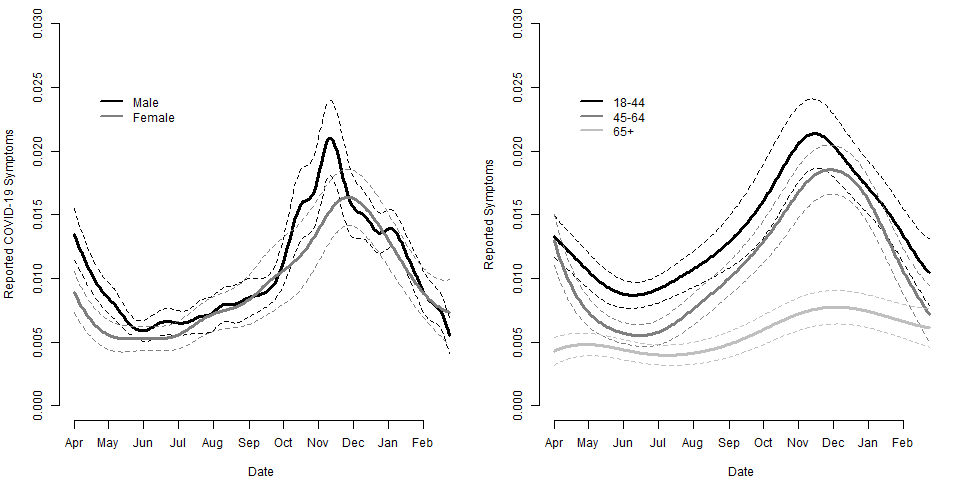
\includegraphics[width = 0.9\textwidth]{../figs/fbcovid19symptoms.png}
\caption{Reported rate of COVID-like symptoms in strata.  Daily rates were estimated using weighted method on each day separately and then smoothed over time using local-linear nonparametric regression.}
\label{fig:fbsymptoms}
\vspace{-0.3cm}
\end{figure}


\section{Analysis of case-count data}
\label{section:casecount}

We start with some simple notation.  Let $N$ denote the population size.  For state-level analysis $N$ is the state's total population, while for country-level analysis $N$ is the country's total population.  At a fixed moment in time, let $Y_j$ denote COVID-19 status for the $j$th individual in the population, $j=1,\ldots, N$. Here, like in survey methodology~\citep{Cochran77}, we treat COVID-19 status as a fixed but unknown quantity of interest. For simplicity, the dynamic nature of the outbreak and recoverability of individuals are initially ignored.  We assume either individual $j$ is COVID-19 positive and $Y_j=1$ or is COVID-19 negative and $Y_j=0$. We also let $I_j \in \{0,1\}$ be an indicator that the individual was selected for testing ($I = 1$) or not ($I=0$).

To start, we assume the primary questions of interest are estimates of the overall number of COVID-19 cases and/or disease prevalence. That is, we are interested in either the population total $Y = \sum_{j=1}^N Y_j$ or the population average $\bar Y = Y/N$. Suppose that $n$ tests are performed and we observe the values $y_1, \ldots, y_n \in \{0,1\}$.  Then a natural candidate for prevalence is the proportion of positive tests $\bar y = \frac{1}{n} \sum_{i=1}^n y_i$, and a natural candidate for overall cases is $N \times \bar y$.
Under simple random sampling (SRS) or any other epsem\footnote{equal probability of selection method} design, the above are unbiased estimators of the population-level quantities of interest.  Under SRS, the variance of the estimator can be expressed as $\frac{1}{N-1} \times \frac{1-f}{f} \times \sigma_Y^2$ where $f = n/N$ is the sampling fraction and $\sigma_Y^2 = \frac{1}{N} \sum_{i=1}^N (Y_i - \bar Y)^2 = \bar Y (1- \bar Y)$.

The above selection mechanisms are random and independent of the outcome of interest. When this is not the case, selection effects may cause bias in the above estimates. To better understand this issue, \cite{Meng2018} provided the following intuitive and powerful statistical decomposition of the error between $\bar y$ and the true proportion $\bar Y$
$$
\bar y_n - \bar Y =  \rho_{I, Y} \times \sqrt{\frac{1-f}{f}} \times \sigma_Y.
$$
The first term represents \emph{data quality}, the second \emph{data quantity}, and the third \emph{problem difficulty}. The term $\rho_{I,Y}$ is the empirical correlation between the population values~$\{ Y_j \}_{j=1}^N$ and the selection values $\{ I_j \}_{j=1}^N$.  Under simple random sampling, $E_{\I} [ \rho_{I,Y} ] = 0$, where the expectation is with respect to the selection mechanism~$\I$, so there is no bias.  The SRS variance formula above shows that $E_{\I} [ \rho_{I,Y}^2 ]  = 1/(N-1)$.

% The key issue with selective testing is that $E_{\I} [ \rho_{I,Y} ] \neq 0$.  Meng identified this as the fundamental issue that can lead to paradoxes in the analysis of big data. The remainder of this paper aims to build upon this fundamental work by extending the decomposition in two directions: accounting for measurement error and the temporal nature of the pandemic.  We then discuss effective sampling methods and their importance in the current pandemic.

\subsection{Imperfect testing}
\label{section:imperfecttesting}

Tests are imperfect.  COVID-19 testing is no exception. Here we investigate the interplay between imperfect testing and selection bias.  In discussions of inaccurate testing, the standard assumption is measurement error leads to parameter attenuation.  When paired with selection bias, however, the two sources of error become entangled, and resulting errors can become magnified, muted, or even switch signs.

First we require some additional notation.  Let $P_j$ be an indicator of measurement error, equal to $1$ when we incorrectly measure the outcome and $0$ when we observe the true outcome. We suppose this is a stochastic variable where $\pr(P_j = 1 \mid Y_j = 1) =: FN$ is the false-negative rate and $\pr(P_j = 1 \mid Y_j = 0) =: FP$ is the false-positive rate.  If individual $j$ is selected (i.e., $I_j = 1$) then the observed outcome can be written as $Y_j^{\star} = Y_j(1-P_j) + (1-Y_j) P_j$.  The attentive data analyst will recognize the estimator $\bar y_n$ is biased even for simple random samples.  In Appendix~\ref{app:memestimator}, assuming sensitivity and specificity were known a priori, we present a novel iterative procedure that uses the error decomposition to construct the estimator $\tilde y_n = (\bar y_n - FP)/(1-(FP+FN))$, which is unbiased under simple random sampling (SRS); see Appendix~\ref{app:modelbased} for a discussion of the connection to model-based estimators. To understand the impact of selection bias and imperfect testing, we derive the following statistical decomposition of the error between $\tilde y_n$ and $\bar Y$:
\begin{equation}
\label{eq:statdecomp}
\rho_{I,Y} \times \sqrt{\frac{1-f}{f}} \times \sigma_{Y}
\times \underbrace{\left[ 1 - \Delta \times \frac{\bar Y}{1-\bar Y} \times \frac{FP(1-\bar Y) + FN \cdot \bar Y}{f_0 (1-\bar Y) + f_1 \bar Y} \right] \times \frac{1}{1-(FP+FN)}}_{D_M},
\end{equation}
where $f=n/N$ is the sampling fraction, $f_1$ and $f_0$ are sampling fractions for COVID-19 positive and negative individuals respectively, and $\Delta = f_1 - f_0$ is the sampling rate differential.  See Appendix~\ref{app:memestimator} for the derivation. This extends work by \cite{Meng2018} to account for imperfect testing. The first term represents \emph{data quality}, the second \emph{data quantity}, and the third \emph{problem difficulty}.  The final term represents the \emph{imperfect testing adjustment} which is again a complex function of the sampling rate differential, the odds ratio, and the ratio of measurement error interaction with prevalence and sampling rates interaction with prevalence but here is scaled by the factor $(1 - FP - FN)^{-1}$ compared to prior decomposition.

Figure~\ref{fig:heatmap} shows that $D_M$, as a function of the relative frequency ($f_1/f_0$) and odds ratio, can be both positive and negative as well as a range of magnitudes~\citep{Beesley2020,Beesley2019,Smeden2019}. Under perfect testing, $D_M = 1$ so the relation between estimation and selection bias is simple, e.g., COVID-19 positive individuals more likely to receive test implies upward bias in prevalence estimates. When tests are imperfect, this simple relationship no longer holds.

\begin{figure}[!th]
\centering
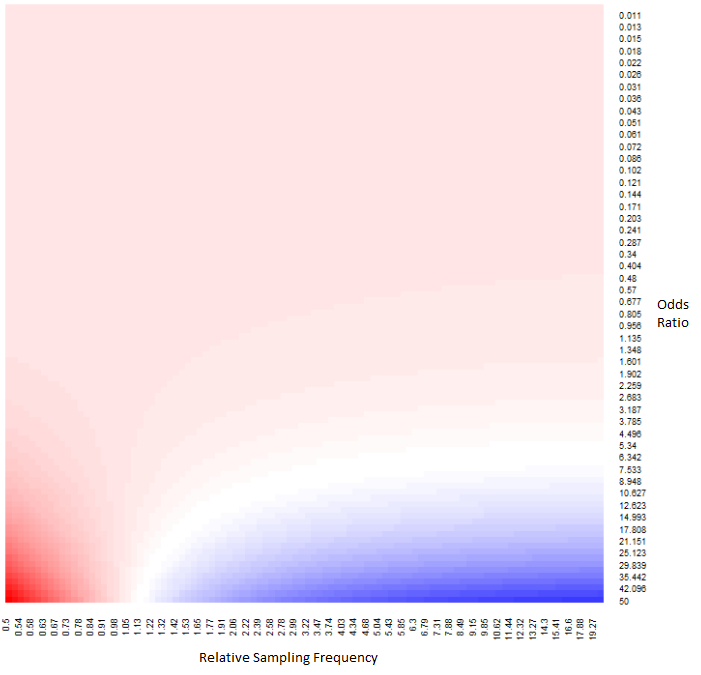
\includegraphics[width = 0.4\textwidth]{../figs/mem_heatmap_article.png}
\caption{Imperfect testing adjustment: relative frequency $f_1/f_0$ (x-axis) against odds ratio (y-axis) for $FP=0.005$ and $FN=0.172$. Color scaled so blue = $-10$, white = $0$, and red = $10$.}
\label{fig:heatmap}
\vspace{-0.3cm}
\end{figure}

Comparing the mean-squared error (MSE) under a selection mechanism $\I$ with imperfect testing and SRS with perfect testing, we see that
$$
\frac{E_{\I} \left[ (\bar y_n - \bar Y)^2 \right]}{\sqrt{V_{SRS} (\bar Y)}} = (N-1) E_{\I} \left[ \rho_{I,Y}^2 D_M^2 \right]
$$
implying the error relative to SRS increases as a function of population size~\citep{Meng2018}. The paradox that two countries with the same testing strategy can yield wildly different estimates due to population size is too often ignored in current communications of case-count data.  When comparing the US and UK under the assumption of similar testing strategies, for example, the MSE increases by a factor of five.  Thus, conclusions drawn from observed case-counts may not just be wrong, but very wrong.

A key question is ``What is the (effective) sample size from a SRS with perfect testing that would yield equivalent MSE to the current testing strategy?'' In Appendix~\ref{app:effss}, we show the effective sample size $n_{eff}$ can be bounded by
$$
\frac{f}{1-f} \times \frac{1}{E_{\I} \left[ \rho_{I,Y}^2 D_M^2 \right]}.
$$
As of June 10th, the US has performed $21,474,531$ tests.  The US population is roughly $312$ million, so $f = 0.069$.  The cumulative empirical prevalence is $9.3\%$ on May 8th. A recent study estimates a false positive and negative rate for antibody testing at $0.5$\% and $17.2$\% respectively \citep{Bendavid2020}. Supposing COVID-19 positive individuals are $2$ times more likely to get tested, then the effective sample size is $92$.  Recent proposals~\citep{Siddarth2020} have argued for increased testing capacity, which may likely reduce the relative sampling rate.  If the relative sampling rate drops to $1.2$ then the effective sample size will increase to $1950$.  Thus the effective sample size even in optimistic scenarios is equivalent to a small random sample from the population.  Moreover, increased testing capacity may also come at the cost of increases in false positive and negative rates.  Consider the case where $f$ increases from $0.05$ to $0.1$ and the increase is associated with the false negative rate rising from $5\%$ to $20$\%.  Then the effective sample size increases by a factor of $1.76$ rather than the expected $4$ fold increase.
% \begin{wrapfigure}{r}{0.5\textwidth}

% {\bf Figure of individual going through the states? Can discuss exposure length as selection more likely.}

\subsection{Regrettable rates: complex biases resulting from self-selection}
\label{section:rates}

The prior analysis demonstrates the limited information regarding COVID-19 prevalence in observational case-count data.  Scientists, however, may claim that daily observed case-counts simply undercount daily total cases by a constant multiple over time.  If true then the ratio of case-counts at consecutive times may be a good estimate of the true change in prevalence, helping scientists understand the disease trajectory.  In this section, we demonstrate how selection bias and imperfect testing impact such estimates.

Let $\bar Y_{t-1}$ and $\bar Y_{t}$ denote the prevalence on two consecutive days and consider the estimator $r = \tilde y_t / \tilde y_{t-1}$.  Using a second-order Taylor series approximation, the error between ${\tilde y_t}/{\tilde y_{t-1}}$ and ${\bar Y_{t}}/{\bar Y_{t-1}}$ can be expressed approximately as
$$
\begin{aligned}
\frac{\bar Y_t}{\bar Y_{t-1}} &\times \bigg[ \rho_{I_t,Y_t} D_{M_t} \sqrt{\frac{1-f_t}{f_t}} CV (Y_t)  -\rho_{I_{t-1},Y_{t-1}} D_{M_{t-1}} \sqrt{\frac{1-f_{t-1}}{f_{t-1}}} CV (Y_{t-1}) \bigg] \\
&\times \left[ 1 - \rho_{I_{t-1},Y_{t-1}} D_{M_{t-1}} \sqrt{\frac{1-f_{t-1}}{f_{t-1}}} CV (Y_{t-1}) \right]
\end{aligned}
$$
where $\rho_{I_j, Y_j}$ is the data quality, $f_j$ is the sampling fraction, $D_{M_j}$ is the measurement error adjustment, and $CV(Y_j) = \sigma_{Y_j}/Y_j$ is the coefficient of variation on day $j$.  See Appendix~\ref{app:ratio} for the derivation. The error magnitude depends on the true rate $\bar Y_{t} / \bar Y_{t-1}$ so a large decrease will have a relatively small error compared to a large increase. The second term represents potential \emph{cancellation} which may occur when data quality, sampling fraction, measurement error, and prevalence are all constant across time.

Figure~\ref{fig:ratio-bias} displays the trajectory of the true ratio and the potential biased estimators under an SIR model~\citep{Pastor2001,Newman2002,Parshani2010} for the epidemic dynamics, with state evolution given by
\begin{equation}
\label{eq:sir}
\frac{\partial s_t}{\partial t} = - \beta s_t i_t; \quad
\frac{\partial i_t}{\partial t} = \beta s_t i_t - \gamma i_t; \quad
\frac{\partial r_t}{\partial t} = - \gamma i_t
\end{equation}
where $s_t$ is the fraction of susceptible individuals, $i_t$ is the fraction of infected individuals, and $r_t$ is the fraction of removed (recovered or deceased) individuals in the population at time $t$.  In terms of bias, the rate is overestimated prior to the peak and underestimated afterwards; the bias increases dramatically when the relative fraction exceeds $2$.  From a decision making perspective, such biases have a substantial impact.  First, the overestimation may give lawmakers and governors more leverage in proposing aggressive actions that reduce prevalence.  Of course, the analysis supports the argument that the estimates based on available data may be pessimistic. What is missing in the current public health discourse is that the bias direction of the prevalence estimate is non-constant over time.   Underestimation post-peak puts pressure on lawmakers and governors to prematurely relax social distancing measures.  Moreover, it appears that the peak time is the easiest to estimate in terms of having minimal error using available data.  Note, however, that the standard errors will be large due to small effective sample sizes.

\subsection{Estimation of effective reproduction number}
\label{section:r0-estimation}
Many epidemiologists argue that tracking the effective reproduction number $R_t$ is the only way to manage through the crisis~\citep{Gabriel2020}.  Under a Poisson likelihood, a simple relation between the trajectory of new cases and the effective reproduction number can be derived \citep{Bettencourt2008}.  In particular, under an SIR model the number of case counts on day $t$, denoted $K_t$, is Poisson distributed with rate $K_{t-1} \exp \left( \gamma (R_t - 1) \right)$ where $K_{t-1} = Y_{t-1}-Y_{t-2}$ is the number of new cases on day $t-1$ and $\gamma$ is the serial interval, which is approximately $7$ days for COVID-19~\citep{Sanche2020}.  Using this relation, a moment-based estimator is given by
$$
R_t = 1 + \frac{1}{\gamma} \log \left( \frac{K_t}{K_{t-1}} \right).
$$
Of course, we do not observe $K_t$ and $K_{t-1}$.  Under SRS of new cases among those susceptible on day $t$, the natural estimator is $S_t \tilde y_t$.  Unfortunately the number of susceptible individuals on day $t$ is unknown.  Here, we study the estimator $\hat R_t = 1 + \frac{1}{\gamma} \log \left( \tilde y_t / \tilde y_{t-1} \right)$. We can again express the statistical error of $\hat R_t - R_t$ in useful terms as follows
$$
\begin{aligned}
\frac{1}{\gamma}\log &\bigg( 1 + \bigg[ \rho_{I_t,K_t} D_{M_t} \sqrt{\frac{1-f_t}{f_t}} CV (K_t)  -\rho_{I_{t-1},K_{t-1}} D_{M_{t-1}} \sqrt{\frac{1-f_{t-1}}{f_{t-1}}} CV (K_{t-1}) \bigg] \\
&\times \left[ 1 - \rho_{I_{t-1},K_{t-1}} D_{M_{t-1}} \sqrt{\frac{1-f_{t-1}}{f_{t-1}}} CV (K_{t-1}) \right] \bigg) - \frac{1}{\gamma} \log \left( \frac{S_t}{S_{t-1}} \right).
\end{aligned}
$$
This implies a similar trade-off as before but on the logarithmic scale.  The error is no longer scaled by $\bar Y_t/\bar Y_{t-1}$ but by the serial interval and does not depend on prevalence $\bar Y_t$ but on the fraction of new cases out of those susceptible $\bar K_t$. This leads to differences in when the bias is most pronounced. The final term is the error due to varying numbers of susceptible individuals.  Figure~\ref{fig:r0-bias} displays the bias as a function of the relative sampling fraction assuming the fraction of the population that is susceptible remains large.

\begin{figure}
\centering
\begin{subfigure}{.5\textwidth}
  \centering
  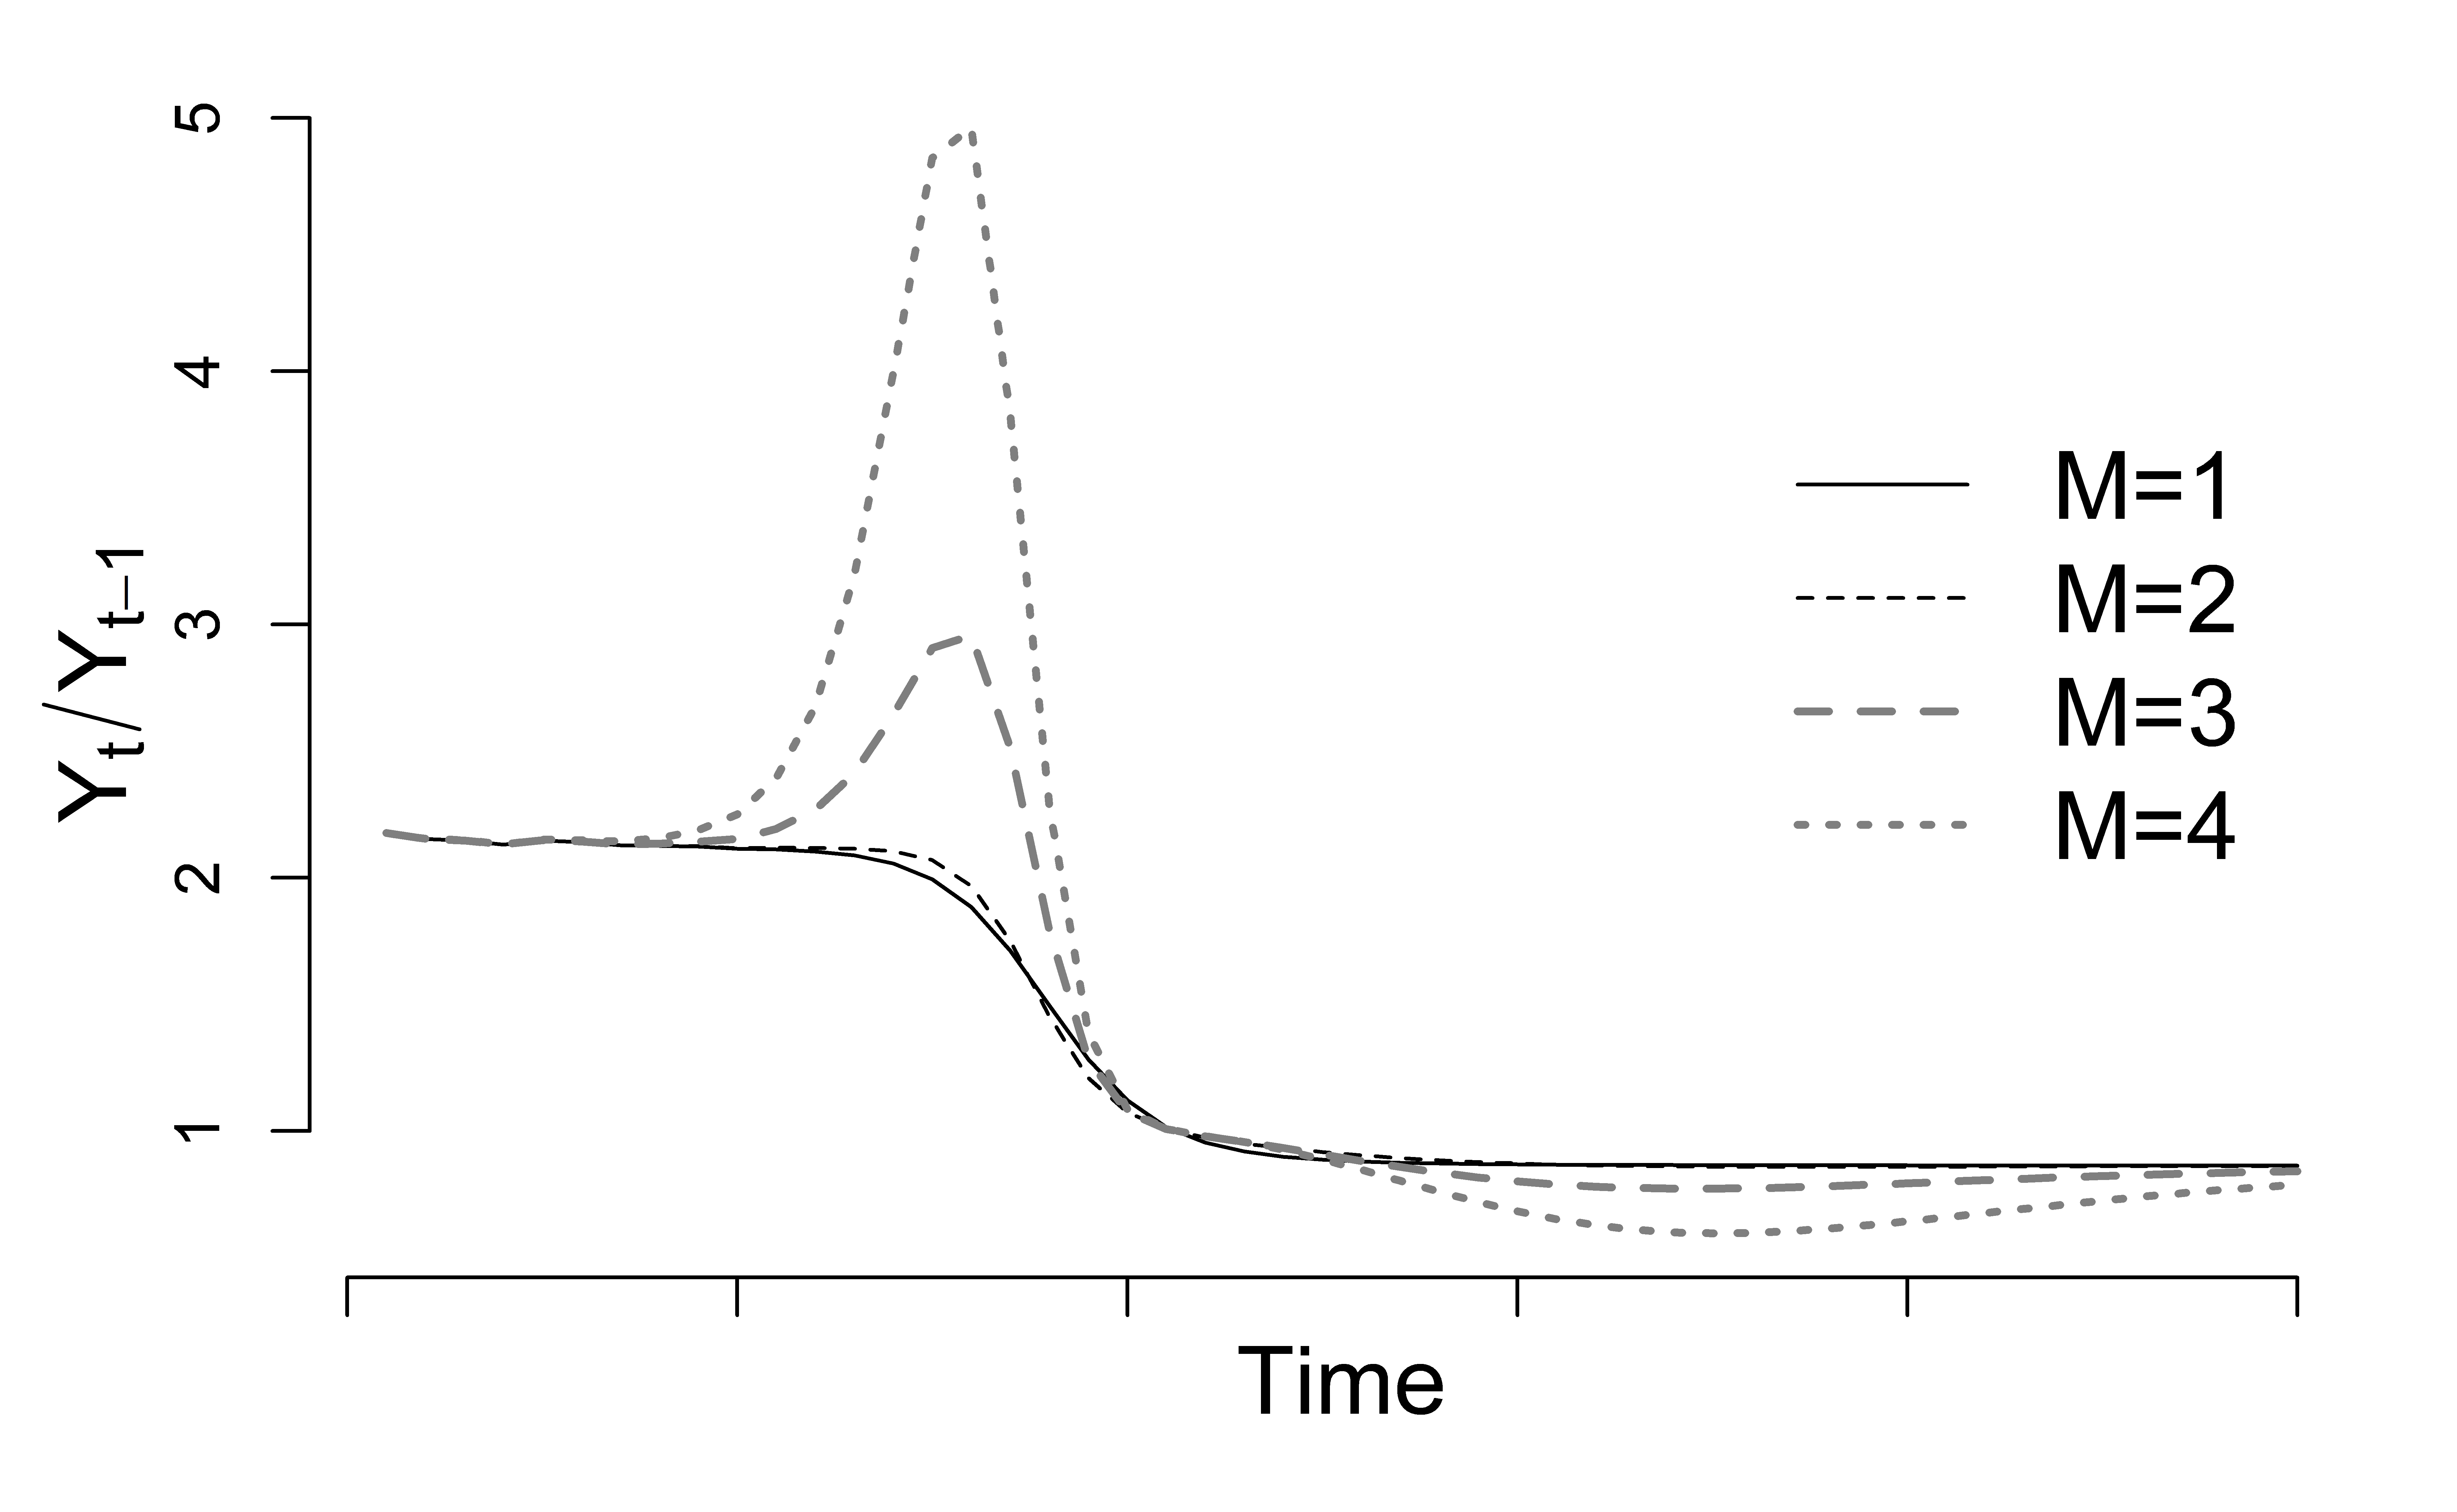
\includegraphics[width=.9\linewidth]{../figs/sir_ratio.png}
  \caption{Ratio estimator}
  \label{fig:ratio-bias}
\end{subfigure}%
\begin{subfigure}{.5\textwidth}
  \centering
  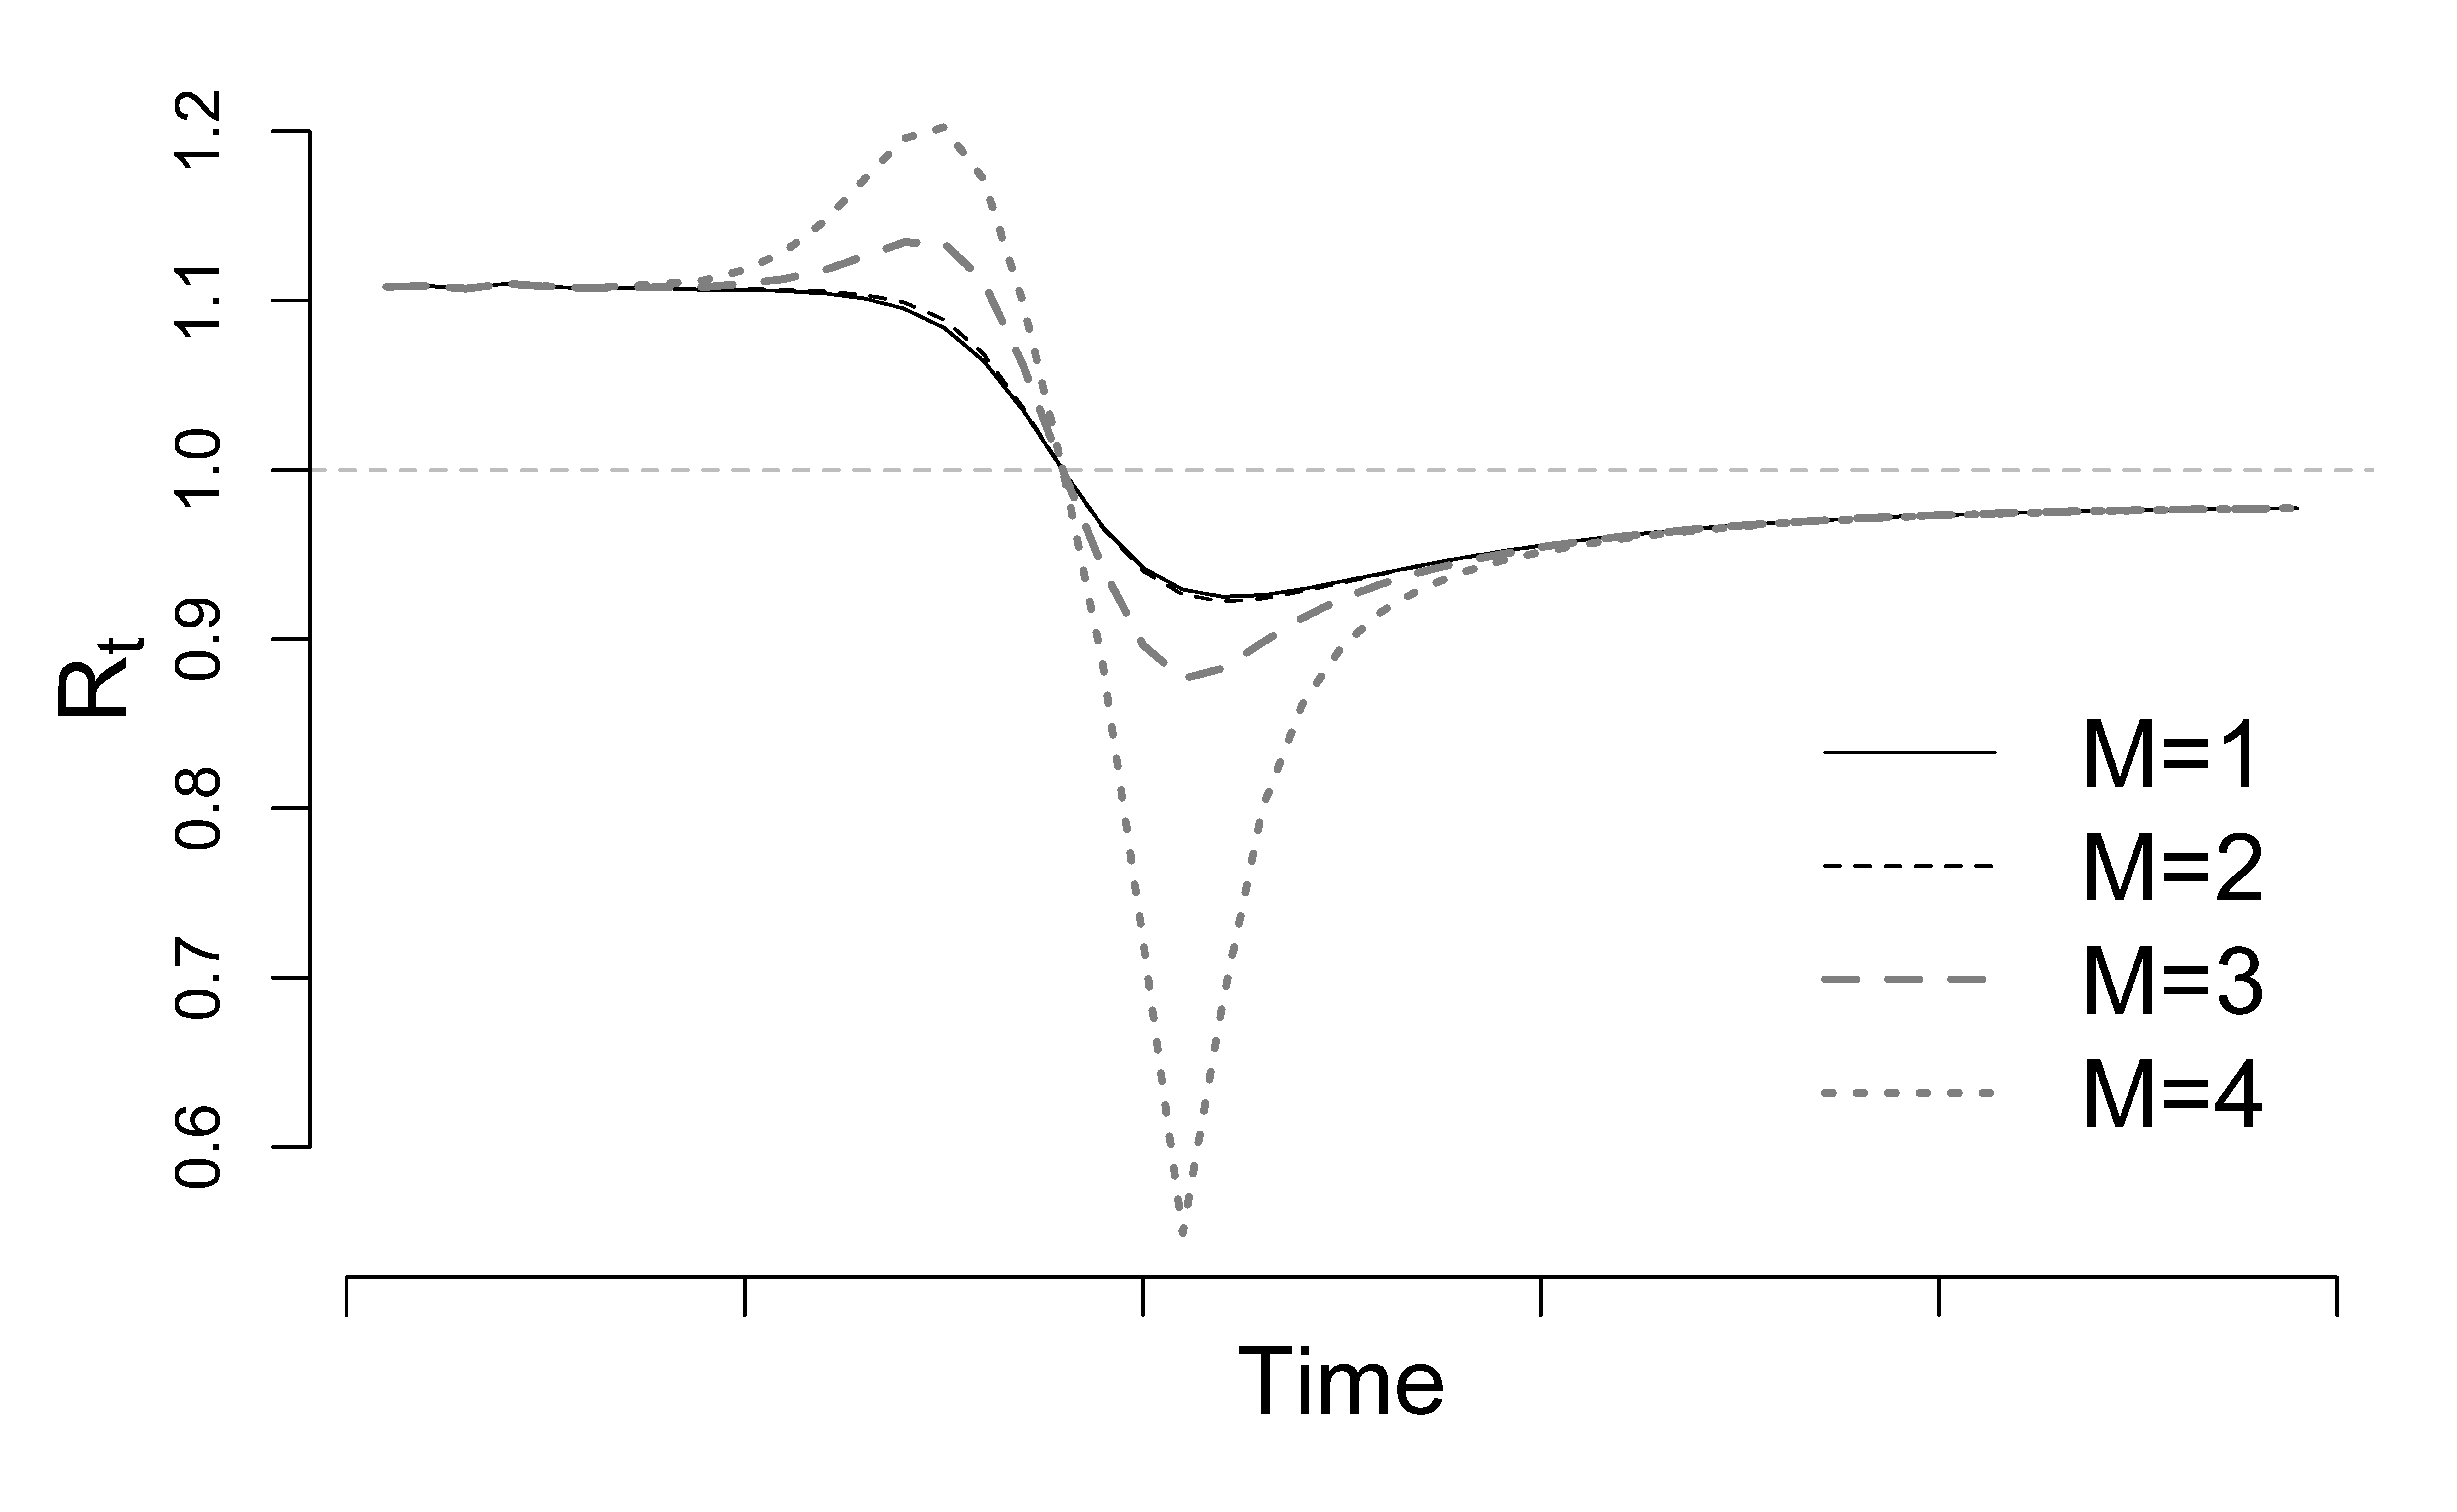
\includegraphics[width=.9\linewidth]{../figs/sir_rt.png}
  \caption{Effective reproductive rate estimator}
  \label{fig:r0-bias}
\end{subfigure}
\caption{Potential bias due to self-selection and measurement error from a deterministic SIR model with $\beta = 1.2$ (black) and $\gamma = 0.15$.  Here we assume $f = 0.02$, $FP = 0.005$, $FN = 0.172$, and use a range of relative sampling fraction $M = f_1/f_0$.}
\label{fig:rates}
\end{figure}

\subsection{Rate comparisons}

So far we have focused on understanding the limitations of using case-count data to understand population quantities of interest for a \emph{single} population.  Many are interested in cross-population comparisons to contrast the impact of countries' mitigation policies.  Here, for simplicity, we focus on comparing the estimated effective reproductive rate.  We assume the two time-series are aligned so that $t=0$ is the time of first case in each population respectively.
% This negates alignment issues and is common in practice.

% While the above issues on $Z$-scores and effective sample size are important, here we highlight a separate issue.
Here we demonstrate the interaction of biases in estimation of the two trajectories when the peak infection times differ slightly.  First, we can write the difference in the rates as
$$
R_{t1} - R_{t2} = \frac{1}{\gamma} \log \left( \frac{1 + e_{1t}}{1+e_{2t}} \right)
$$
where $e_{jt}$ is the error associated given in Section \ref{section:r0-estimation}.  Recall that the error allowed for over-estimation prior to the peak and then under-estimation post-peak.  Here, these errors can mingle in interesting ways.  Consider two countries (A and B) in which the peak occurs 2 weeks prior for country A than country B.  Figure~\ref{fig:comparison} presents such a comparison where each country's disease trajectory follows an SIR model (A=black and B=red). Of interest is the difference between the effective reproduction rate for country A and B, $R_{tA} - R_{tB}$. Figure~\ref{fig:eff} shows how biases in estimation of each rate interact in complex ways.  At first, the difference is correctly estimated; then the gap is over-estimated as country A sees a rapid rise in cases; then the magnitude of over-estimation increases as country A sees declining case-count while country B sees rapidly increasing case-count; then country A's rate is correctly estimated while country B's rate is under-estimated as it sees declining case-count; finally, the gap disappears.  We do not claim this will always be the case; however, this demonstrates how observed information can tell a more complex story than the truth (i.e., country A's peak is 2 weeks prior to country B's peak).

\begin{figure}
\centering
\begin{subfigure}{.5\textwidth}
  \centering
  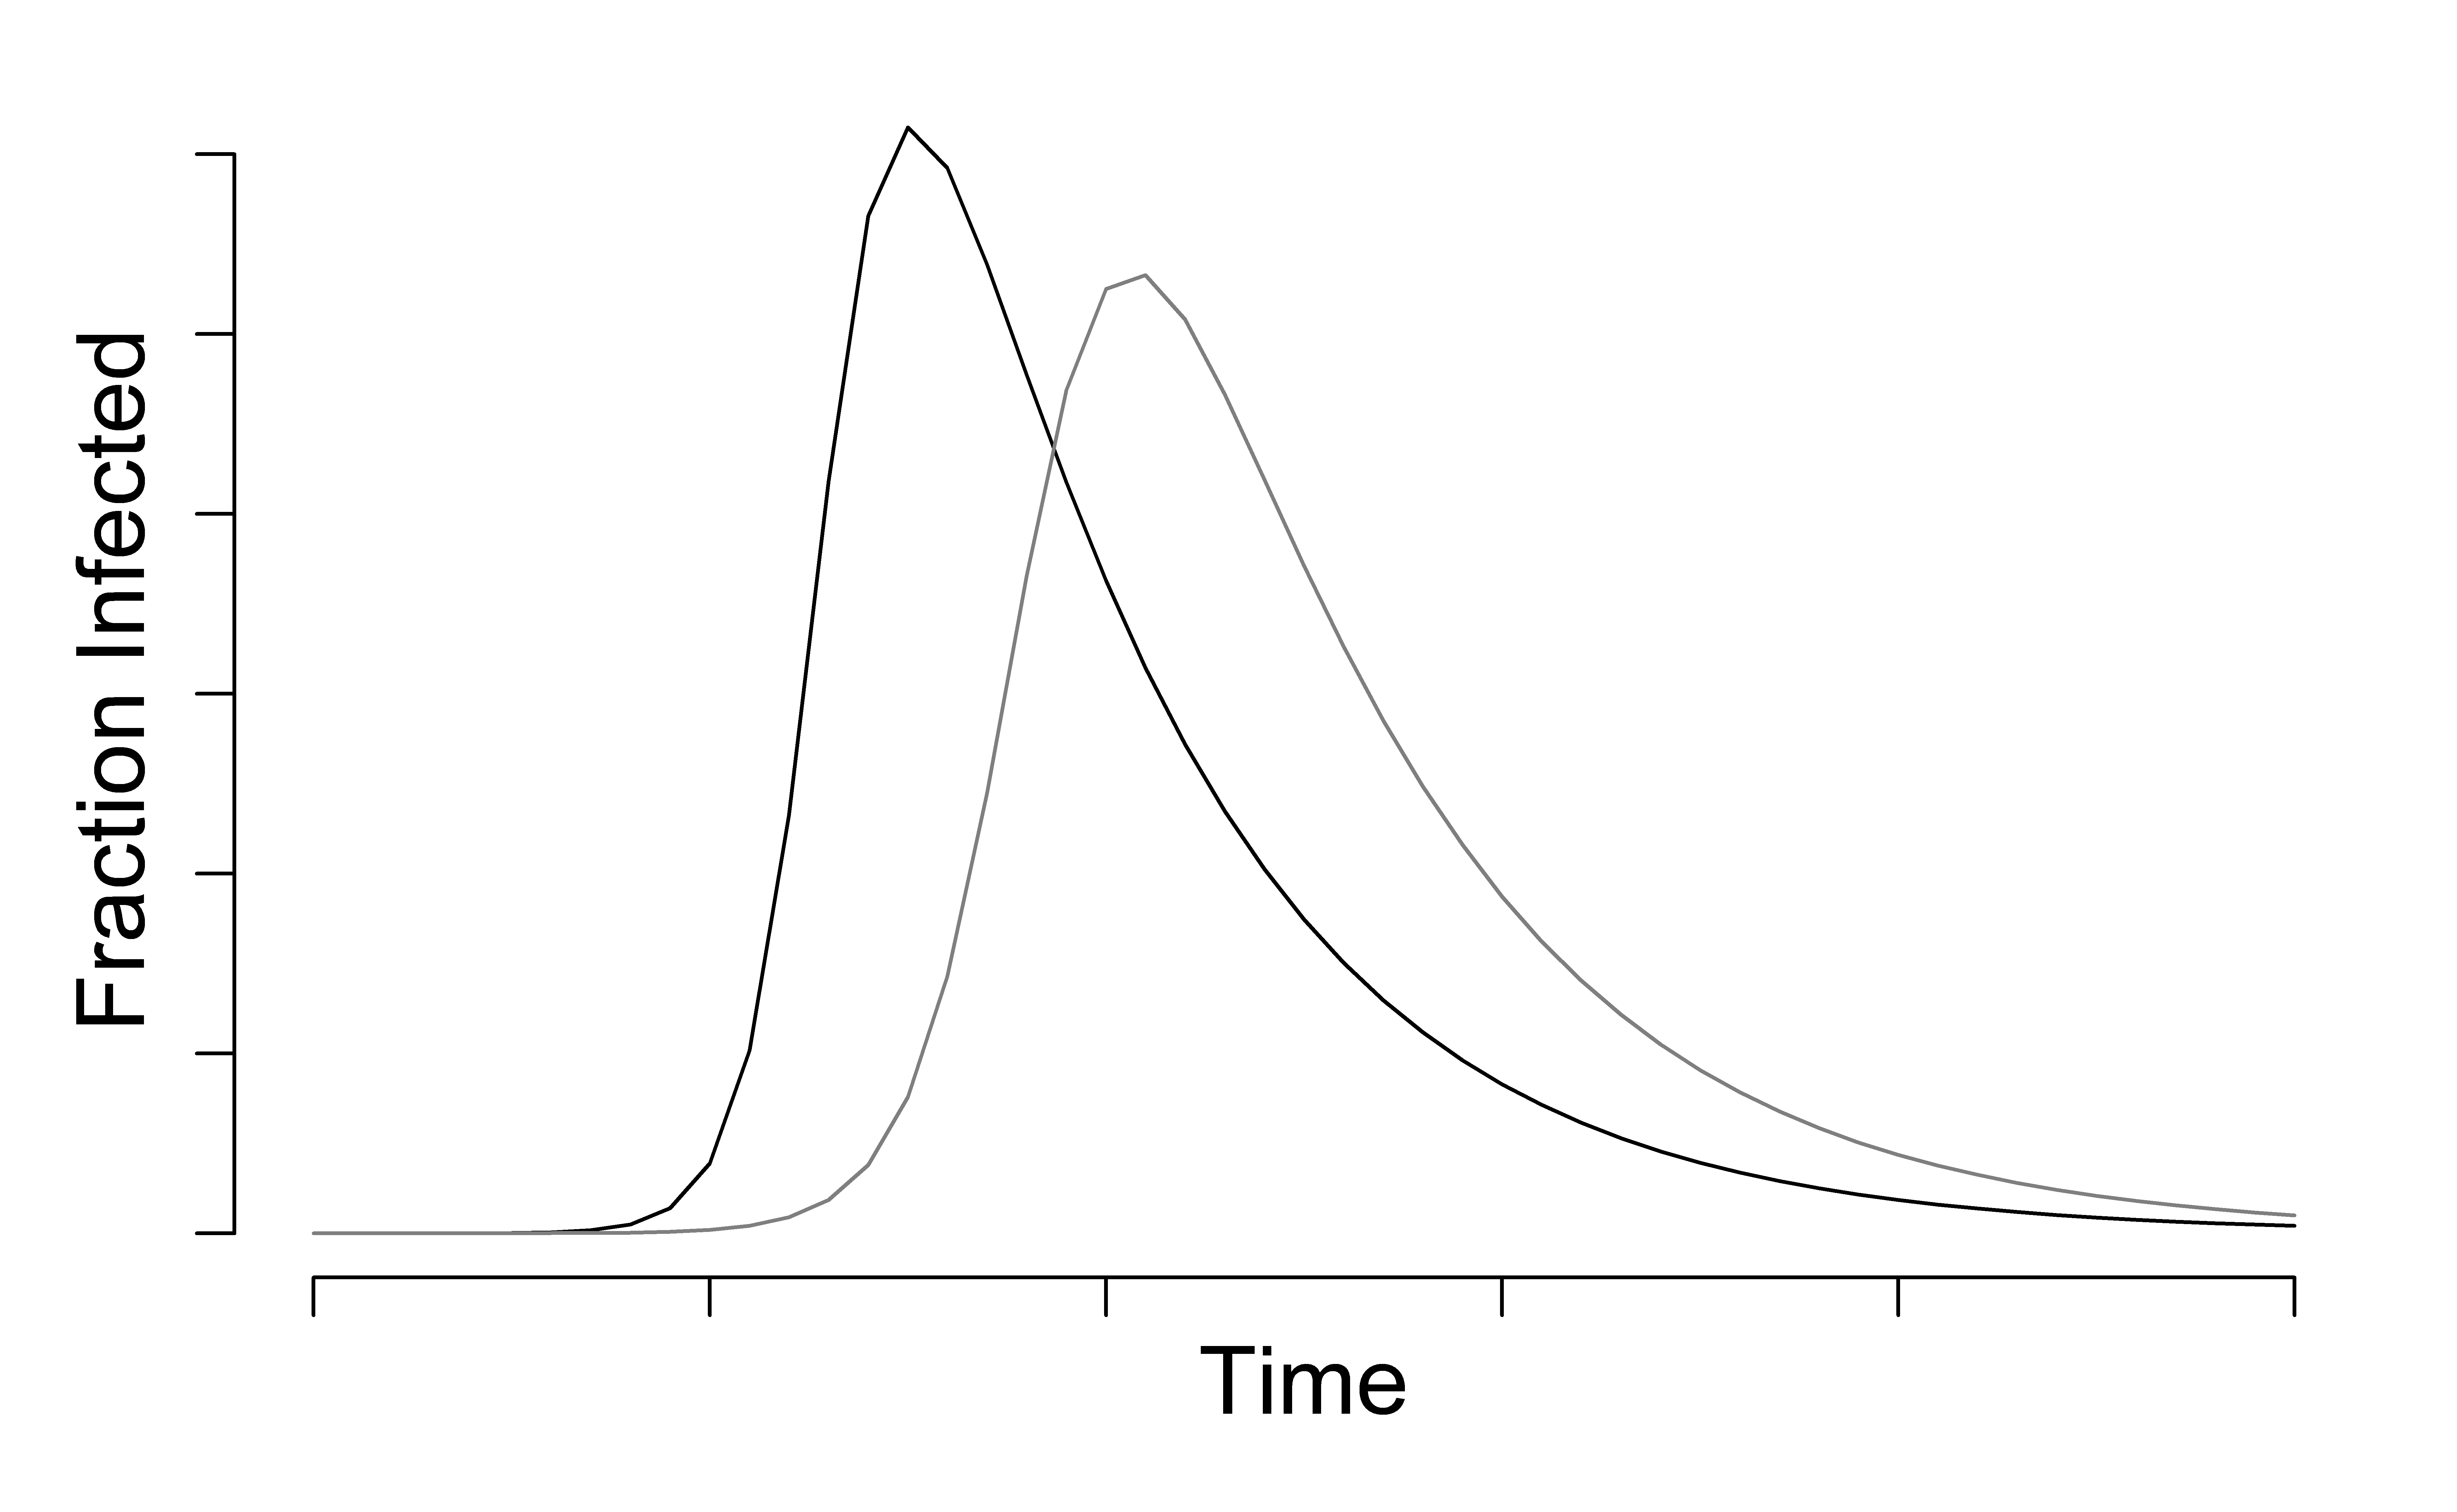
\includegraphics[width=.9\linewidth]{../figs/sir.png}
  \caption{Fraction of new cases in population}
  \label{fig:fracpop}
\end{subfigure}%
\begin{subfigure}{.5\textwidth}
  \centering
  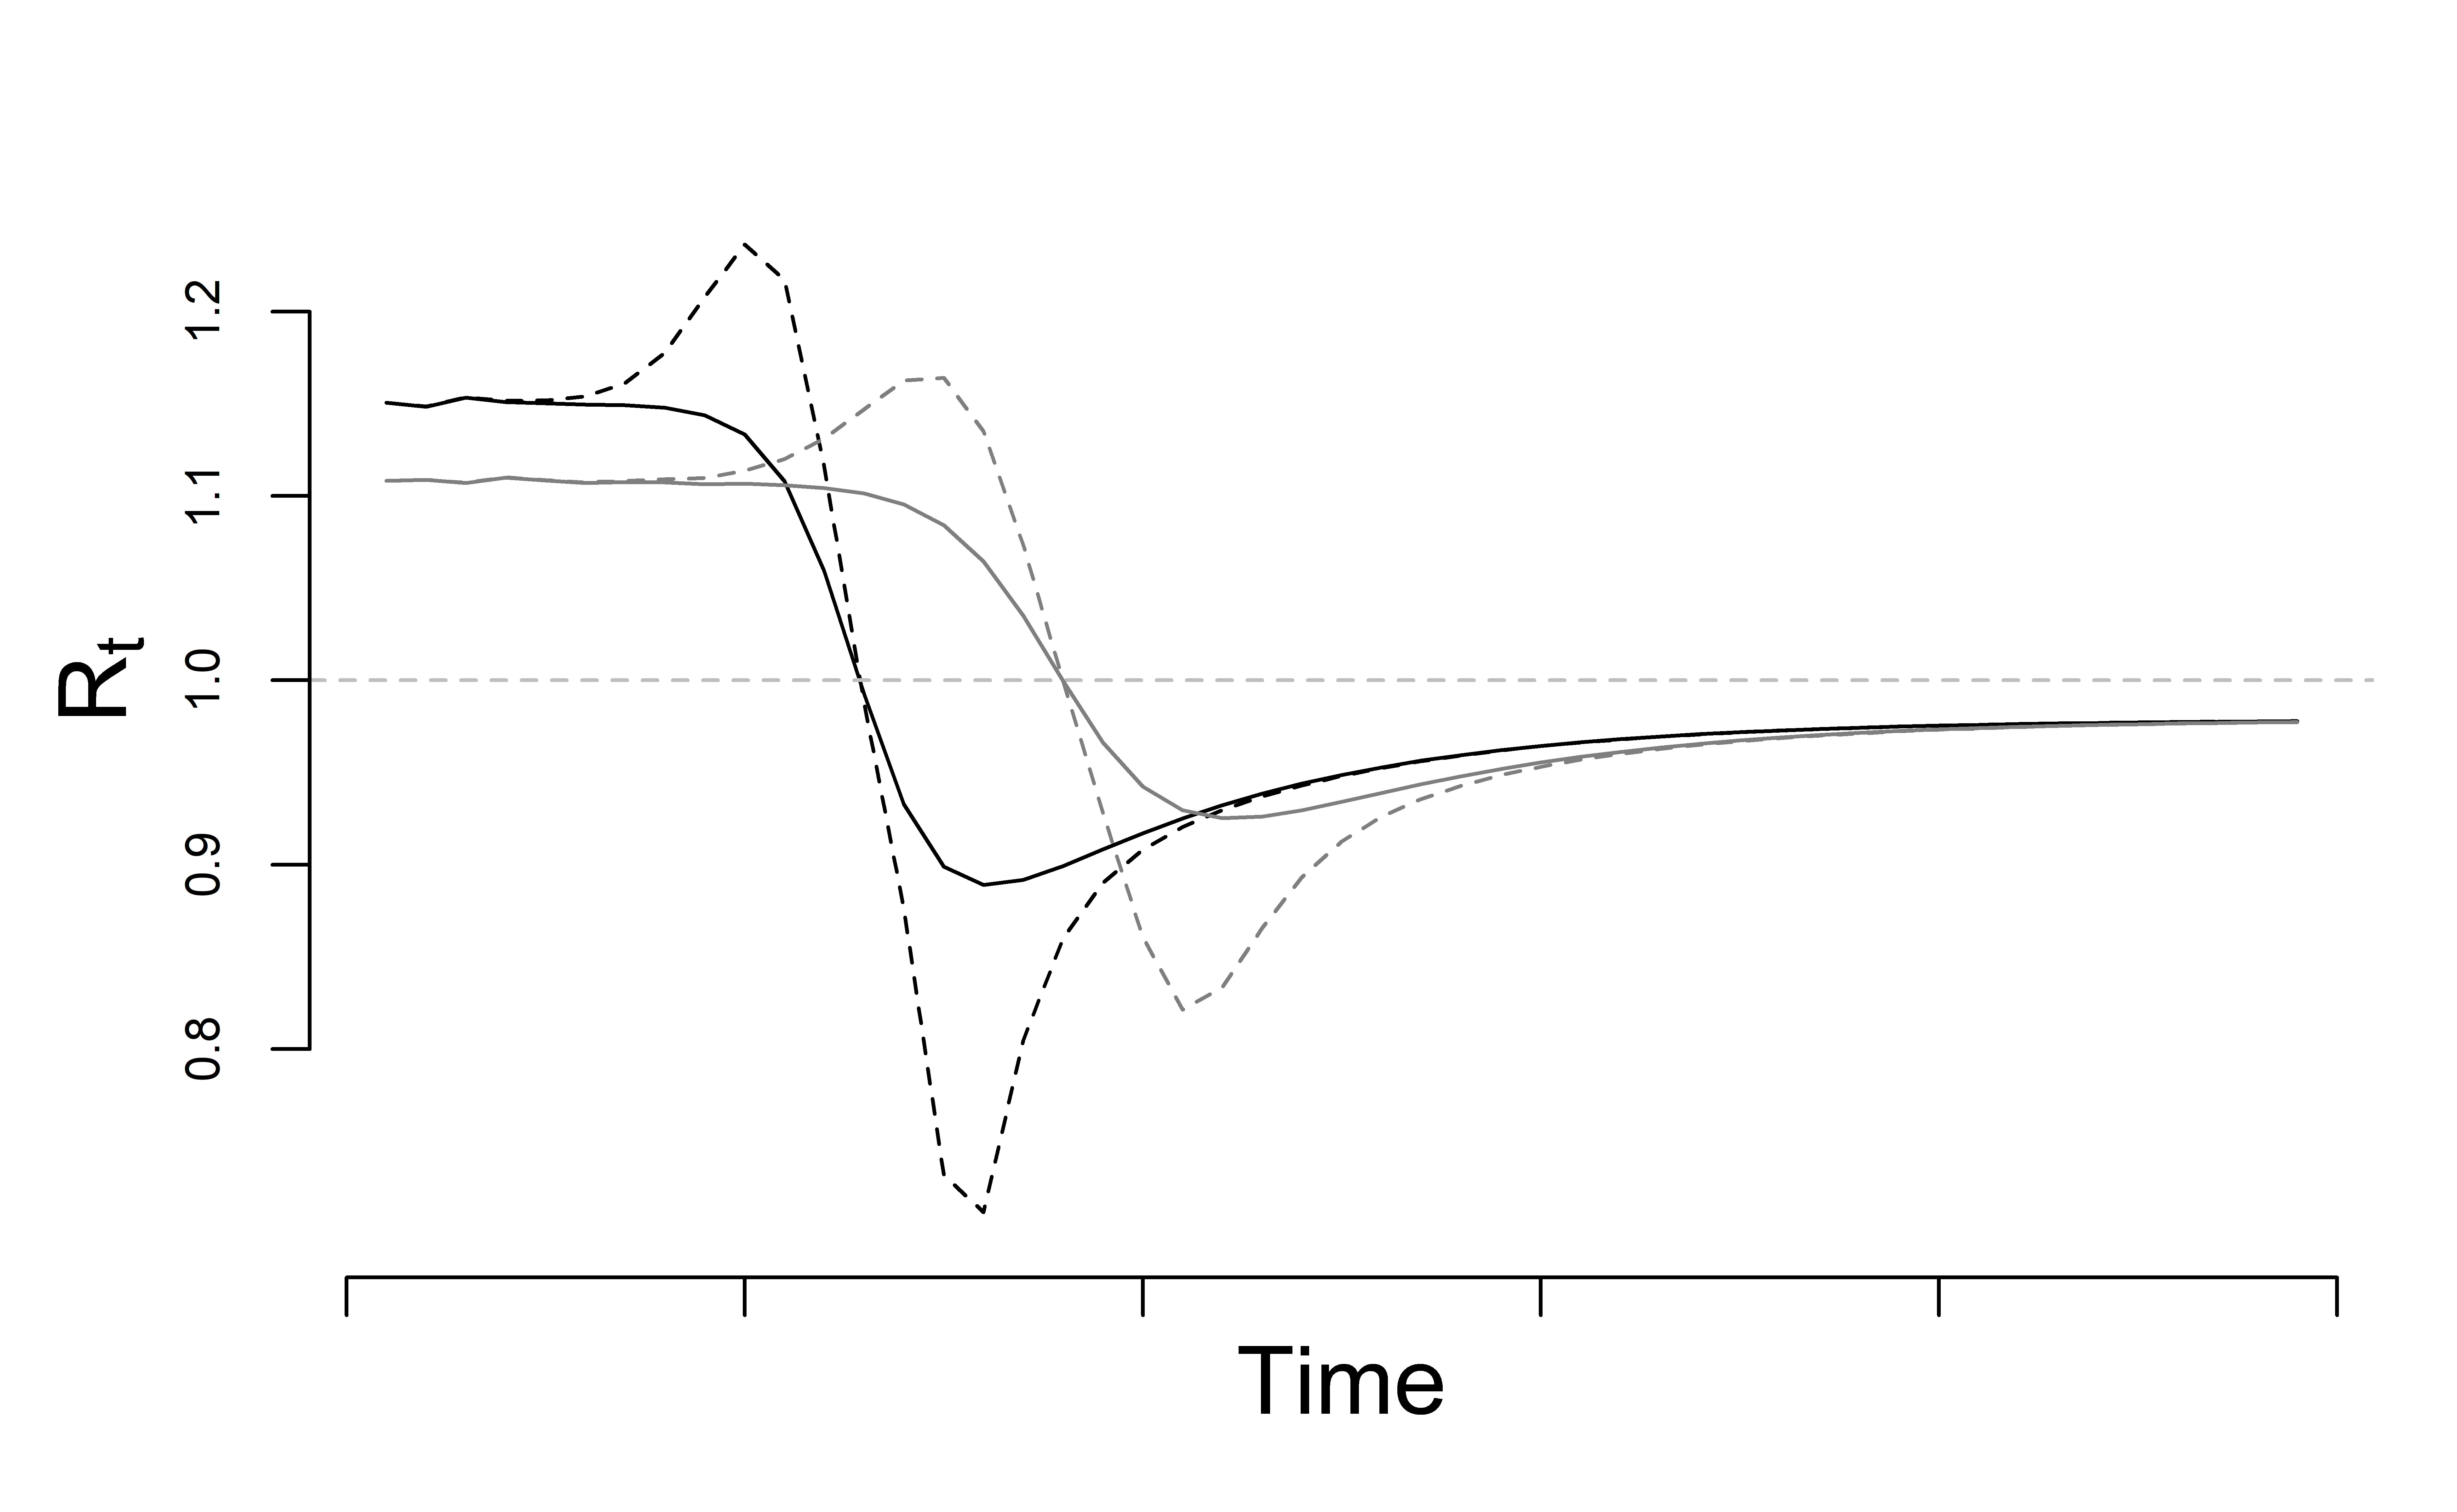
\includegraphics[width=.9\linewidth]{../figs/sir_rt_comparison.png}
  \caption{Effective reproduction rate estimators}
  \label{fig:eff}
\end{subfigure}
\caption{Left: fraction infected in two SIR models with $\beta = 1.2$ and $0.9$ respectively and $\gamma = 0.15$ with same initial conditions. Right: comparison of $\hat R_t$ across time with $FN = 0.172$, $FP = 0.005$, and $M = 4$.}
\label{fig:comparison}
\end{figure}

\section{Potential improvements to prevalence estimation}
\label{section:improvedcasecount}

The prior section presented negative consequences of selection-bias and measurement error when estimating infection prevalence from observed case-count data.  This raises the immediate question whether prevalence estimators can be improved.  In this section, we consider two directions.
% First, we use publicly available auxiliary information to build selection propensities and consider an inverse probability weighting (IPW) estimator. We then extend the statistical error decomposition to the weighted setting. Second, we consider an extension of compartmental models from infectious disease epidemiology using death data.  After adjusting for measurement-error, this leads to an alternative, model-based forecast of prevalence. We then combine these epidemiological forecasts, selection propensities, and measurement-error corrections to generate \emph{doubly robust} prevalence estimators. We provide an appropriate extension of the statistical error decomposition.
The proposed methods and statistical error decompositions guide our recommendations in Section~\ref{section:discussion}.

\subsection{Selection propensity estimation}

With non-probability samples, one can reduce bias by modelling the self-selection propensity and use inverse probability weighting (IPW)~\citep{Elliott2017} techniques to adjust for selection bias.  In causal inference~\citep{Hernan2020}, under certain assumptions, the observational data permits direct estimation of treatment propensity.  In the COVID-19 context, one does not observe those who decide not to be tested.  In order to estimate selection propensities, one needs auxiliary information.

To see this mathematically, let $X_j$ denote a vector of covariates for the $j$th individual in the population, $j=1,\ldots,N$.  For simplicity, the dynamic nature of the outbreak and recoverability of individuals is ignored for now. Suppose the selection indicator $I_j$ is a Bernoulli random variable that depends only on these covariates, i.e., $P(I_j = 1 \mid X_j = x) = \pi (x; \theta)$. Maximum likelihood estimation follows by maximizing
\begin{equation}
\label{eq:propensity}
\sum_{j=1}^N I_j \log \left( \frac{\pi (X_j; \theta)}{1-\pi(X_j; \theta)} \right) + \sum_{j=1}^N \log \left( 1 - \pi (X_j; \theta) \right).
\end{equation}
The first sum only involves individuals observed in the nonprobability sample.
The second sum is over the entire population.  Maximum likelihood estimation therefore requires knowledge of covariate information for every individual in the population.  Typically, this is not possible.  Here we present a method that uses auxiliary information obtained from probability samples as well as probability subsamples from the self-selected population.

\subsubsection{Auxiliary information through probability samples}
\label{subsec:auxprob}

Here, we assume access to a probability sample from the same population on which the outcome and exact same set of covariates are measured.  Let $\tilde I_j$ be an indicator that the individual was included in the probability sample and $\tilde W_j$ be the probability of inclusion for the $j$th individual (i.e., equal to $n/N$ for a simple random sample of size $n$). The probability sample is used to construct a design-unbiased estimator of the second term
\begin{equation}
\label{eq:auxinfoprob}
\sum_{j=1}^N I_j \log \left( \frac{\pi (X_j; \theta)}{1-\pi(X_j; \theta)} \right)  + \sum_{i=1}^N \tilde I_j \tilde W_j \log ( 1 - \pi (X_j; \theta)).
\end{equation}
Taking the expectation of the second term with respect to the sampling design yields the second term in~\eqref{eq:propensity}.  This was proposed by~\cite{Chen2019} when covariates were observed on a random sample from the population.
% Under simple random sampling and non-parametric selection propensity on a stratification variable, the weight is given by estimator of the $\hat \pi_k = (d_k / \tilde d_k) (n / N)$ where $\tilde d_k$ is the number of observations in strata $k$ in the random sample.

% Equation~\eqref{eq:auxinfoprob} presupposes covariate information is collected for all individuals in the nonprobability sample; however, this is often not feasible for state and local governments where rapid sample collection is prioritized over additional collection of covariate information.  We can extend~\eqref{eq:auxinfoprob} by randomly sampling a subset of the nonprobability sample on which to collect the covariate information, yielding the pseudo-likelihood
% \begin{equation}
% \label{eq:auxinfoprob2}
% \sum_{j=1}^N I_j I_j^{(2)} W_j^{(2)} \log \left( \frac{\pi (X_j; \theta)}{1-\pi(X_j; \theta)} \right)  + \sum_{i=1}^N \tilde I_j \tilde W_j \log ( 1 - \pi (X_j; \theta)).
% \end{equation}
% Here, $I_j^{(2)}$ is an indicator that the individual is in the probability subsample and $W_j^{(2)}$ is the probability of inclusion.  Estimation proceeds by maximizing the pseudo-likelihood which now depends on random sampling in both the first and second term.

\subsubsection{An IPW estimator and statistical error decomposition}
\label{section:IPWerrordecomp}

Given a selection propensity, define the inverse probability weight~$w(x) = \pi (x; \hat \theta)^{-1}$. Then the IPW estimator adjusted for measurement error is given by
\begin{equation}
\label{eq:ipwest}
\bar y_n^\star
= \frac{1}{1-FP-FN} \cdot \frac{\sum_{i=1}^n w(x_i) (y_i - FP)}{\sum_{i=1}^n w (x_i)}
\stackrel{(2)}{=} \frac{1}{1-FP-FN} \sum_{k=1}^K \frac{d_k w_k}{w} (\bar y_k - FP),
\end{equation}
where equality (2) is under the assumption that $x_i$ is a stratification variable with $k$ indexing the strata, $w_k$ is the weight and $d_k$ is the number of samples in strata $k$, and $w = \sum_{k=1}^K d_k w_k$. Under simple random sampling with one strata~$\hat \pi_k = n/N$ and we recover the estimator $\tilde y_n$ from Section~\ref{section:imperfecttesting}.

Let $\tilde I_j (X_j) = I_j  \cdot W(X_j)$ for $j=1,\ldots,N$.  Then the error when comparing weighted estimator~$\bar y_n^\star$ to the true prevalence $\bar Y$ can be expressed as:
\begin{equation}
\label{eq:statdecomp2}
\rho_{\tilde I (X), Y} \times \sqrt{\frac{1-f+ CV^2_W}{f}} \times \sigma_{Y} \times \underbrace{\left[ 1 - \tilde \Delta \times \frac{\bar Y}{1-\bar Y} \times \frac{FP(1-\bar Y) + FN \cdot \bar Y}{\tilde f_0 (1-\bar Y) + \tilde f_1 \bar Y} \right] \times \frac{1}{1-(FP+FN)}}_{\tilde D_M}
\end{equation}
where $CV_W$ is the coefficient of variation (i.e., standard deviation/mean) of $W_J$ given $I_J = 1$, $\rho_{\tilde I(X), Y}$ is the empirical correlation which here depends on covariate distribution, $\tilde f_k = E[ W_J I_J \mid Y_j = k]$ for $k=0,1$, and $\tilde \Delta = \tilde f_1 - \tilde f_0$.  See Appendix~\ref{app:ipwderivation} for the derivation.

Comparing~\eqref{eq:statdecomp2} to~\eqref{eq:statdecomp} shows that weighting impacts the estimation error in three ways.  First, there is a negative impact on the data quantity component; taking the ratio of these quantities yields
$\sqrt{1 + \frac{CV_W^2}{1-f}} \geq 1$.  Hence, if the data quality does not increase (i.e., $| \rho_{\tilde I (X), Y} | = | \rho_{I,Y}|$ ) then weighting increases the error magnitude.  Note this relative error increase depends on the fraction of population sampled $f$, implying that for large samples there is a larger potential increase in the error if the weights do not improve data quality. Third, the impact of measurement-error on data quality is changed when considering a weighted estimand. In particular, weighting may result in $\text{sgn}(\Delta) \neq \text{sgn} (\tilde \Delta)$ which implies the impact of measurement-error may be in a different direction.

As demonstrated in Lemma~\ref{lemma:ipw}, if the propensity model is correctly specified then the $E_{\bf R} [ \rho_{\tilde I (X), Y} ] = 0$ and therefore $\rho_{\tilde I(X), Y} = O(N^{-1})$; however, if the weights are not correctly specified then the data quality index is unlikely to inversely scale with population size.  Indeed, Horvitz-Thompson estimators are sensitive to errors in the estimated weights.  Low selection propensity imply large weights which can have deleterious impacts by certain observations dominating estimation.   Similar to~\cite{Meng2018}, if the data quality is not at the level of $N^{-1}$, then confidence intervals constructed from an IPW estimator are likely to put too much confidence in the sheer size of the data.

\subsubsection{Time-varying propensities}

In prior sections on selection propensity estimation, we ignored the dynamic nature of the outbreak.  Here we extend the IPW approach to the temporal setting by considering the joint likelihood
\begin{equation}
\label{eq:tvpropensity}
\sum_{t=1}^T \left[ \sum_{j=1}^N I_{j,t} \log \left( \frac{\pi_t (X_{j,t}; \theta)}{1-\pi_t(X_{j,t}; \theta)} \right) + \sum_{j=1}^N \log \left( 1 - \pi_t (X_{j,t}; \theta) \right) \right]
\end{equation}
where $t=1,\ldots,T$ are the days when case-count data is reported.  Here, $I_{j,t}$ denotes self-selection into testing on day $t$, which is highly correlated with prior testing and results.  For example, an individual who tests positive is unlikely to seek testing on subsequent days.  Moreover, an individual in a high prevalence area may be more likely to seek out testing.  Here, we assume that the covariate vector $X_{j,t}$ contains all features of past relevant for selection.

If sufficiently large random samples are collected at each time $t =1,\ldots,T$, then the pseudo-likelihood can be re-written as in~\eqref{eq:auxinfoprob} and propensities estimated separately per time point.  Unfortunately for COVID-19, large probabilistic samples are not available at every time within a given region.  For simplicity, here we discuss a non-parametric kernel-based approach where the selection propensity at time~$t$, denoted $\hat \theta_t$, maximizes the smoothed pseudo-likelihood
$$
\sum_{t^\prime=1}^T K_h(|t^\prime - t|) \left[ \sum_{j=1}^N I_{j,t^\prime} \log \left( \frac{\pi_t (X_{j,t^\prime}; \theta)}{1-\pi_t(X_{j,t^\prime}; \theta)} \right) + \sum_{j=1}^N \tilde W_{j,t^\prime} \tilde I_{j,t^\prime} \log \left( 1 - \pi_t (X_{j,t^\prime}; \theta) \right) \right]
$$
where $K_h$ is a kernel function with tunable parameter $h$. Given $\pi (x;\hat \theta_t)$, the prevalence estimator $\bar y_{n,t}^\star$ is given by~\ref{eq:ipwest}.

% Under simple random sampling of equal size~$\tilde n$ from a fixed population size~$N$ at each time and non-parametric selection propensity on a stratification variable, the weight is given by estimator of the
% $$
% \hat \pi_{k,t} = \frac{n}{N} \times \frac{\sum_{t^\prime=1}^T K_h(|t^\prime - t|) \hat d_{k,t^\prime}}{\sum_{t^\prime=1}^T K_h(|t^\prime - t|) \tilde d_{k,t^\prime}}
% $$
% where $\tilde d_k$ is the number of observations in strata $k$ in the random sample.

\subsubsection{Uncertain sensitivity and specificity}

For prevalence there is some

For

For seroprevalence, \cite{Bendavid2020} report



, which leads to a range for $M$ of $(2.21, 2.38)$.  Therefore, the impact on bias of $\hat R_t$ appears moderate.  If $FP = 0.05$ and $FN = 0.005$, then the relative sampling rate increases to $M=3.04$.  This simple tool helps us understand how sensitivity and specificity impact biases and  therefore how much we should trust conclusions based on these assumptions.


\subsubsection{Asymptotics}

Assuming the selection propensity model is correctly specified, then under the design of the probability sample and design of the subsample from the nonprobability sample, Lemma~\ref{lemma:ipw} shows that the IPW estimator is  consistent and calculates the estimator's variance.  In Lemma~\ref{lemma:ipw}, sensitivity and specificity are not assumed known.  Instead, we suppose that these are estimated using a pseudo-likelihood on a random sample from the population whose size is chosen so the resulting estimated sensitivity and specificity have desired levels of uncertainty.  See Appendix~\ref{app:asympderivations} for additional details.

\begin{lemma}[Variance of IPW estimator] \normalfont
\label{lemma:ipw}
\textcolor{red}{Must check.}
The estimates~$\mu_t := \bar y_{n,t}^\star$ and $\hat \pi_{j,t}$
are solutions to the following set of estimating equations
$$
\Phi_n (\eta_t) =
\left (
\begin{array}{c}
\frac{1}{N} \sum_{j=1}^N I_{j,t} \frac{Y_{j,t} - (1-FP-FN) \cdot (\mu_t+FP)}{\pi_{j,t}} \\
\frac{1}{N} \sum_{t^\prime = 1}^T K_{t,t^\prime} \sum_{j=1}^N I_{j,t^\prime} X_{j,t^\prime} - \frac{1}{N} \sum_{j = 1}^N \tilde I_{j,t^\prime} \tilde W_{j,t^\prime}  \pi_{j,t^\prime} X_{j,t^\prime}  \\
\frac{1}{n_{FP}} \sum_{j \in S_{FP}} \frac{Z_j}{FP} - \frac{1-Z_j}{1-FP} \\
\frac{1}{n_{FN}} \sum_{j \in S_{FN}} \frac{\tilde Z_j}{FN} - \frac{1-\tilde Z_j}{1-FN} \\
\end{array}
\right ) = {\bf 0}
$$
where $\eta_t = (\mu_t, \pi_t, FP, FN)$. Under regularity assumptions (see Appendix~\ref{app:asympderivations}), we have $\bar y_{n,t}^\star - \bar Y_{t} = O_p (n^{-1/2})$ (check)  and $\text{var} (\hat y_{n,t}) = V_{t}^{(IPW)} + o (n^{-1})$ where $V_t^{(IPW)}$ is the first diagonal element of $E [\phi_n(\eta_0)]^{-1} \text{Var}(\Phi_n(\eta_0))E [\phi_n(\eta_0)]^{-1}$.
\end{lemma}

\subsection{Model-based estimation}
\label{section:modelbased}

Up to this point, the primary focus of this paper has been on selection bias in coronavirus case-count data from a survey sampling perspective.  Here, we consider compartmental model approaches from infectious disease epidemiology.  Our primary objective is a model-based forecast of strata-level prevalence $\bar y_k$. To do this, an extension of a standard epidemiological state-space model -- the susceptible, infected, and removed (recovered and death) model, or SIR model -- is presented. Here we consider the probabilistic SIR model was originally proposed by~\cite{Osthus2017} with only one-dimensional time series of infected proportions; this formulation was extended by~\cite{Song2020} to model coronavirus case-counts.

Let $s_t$, $e_t$, $i_t^{(T)}$, $i^{(NT)}$, and $r_t$ denote the proportion of survivors, exposed, currently transmitting and not trasmitting infected, and removed cases (i.e., including both recovered cases and deaths) at time $t$.  Suppose $K$ strata such that the proportions are defined per strata, i.e., $s_t = (s_{1,t},\ldots, s_{K,t})$ is the proportion of survivors in each strata. Let $\theta_t = (s_t, e_t, i_t^{(T)}, i_t^{(NT)}, r_t)$, then we assume the process is governed by the following Markov model:
$$
\theta_t \mid \theta_{t-1}; \tau \sim \text{Dirichlet} \left(\kappa f(\theta_{t-1}, \beta, \gamma) \right)
$$
where $\kappa$ scales the variance of the Dirichlet distribution and $f(\cdot)$ is a function that determines infection dynamics.  Here, we extend the SIR dynamics to account for strata-level dynamics
\begin{align*}
\frac{\partial s_t}{\partial t} &= - s_t \circ (B \, i^{(T)}_t); \quad \frac{\partial e_t}{\partial t} = s_t \circ (B \, i^{(T)}_t) - \sigma e_t; \quad \\
\frac{\partial i^{(T)}_t}{\partial t} &= \sigma e_t - \beta_2 i^{(T)}; \quad
\frac{\partial i^{(NT)}_t}{\partial t} = \beta_2 i^{(NT)}  - \gamma i^{(NT)}; \quad \\
\frac{\partial r_t}{\partial t} &= - \gamma i^{(NT)}_t
\end{align*}
where $B \in \mathbb{R}^{K \times K}$ and $\circ$ denotes elementwise product of vectors.  The matrix $B$ allows for strata-specific infection dynamics with the SIR model being recovered if $B_{k,\cdot} = \beta$ for each $k \in [K]$.  Following~\cite{Song2020}, we employ Runge-Kutta (RK4) approximations for discretization; see Appendix XX for details.

Selection bias in case count data could be direcly addressed by extending the above compartmental model.  Here, we instead opt to bring in a different source of information by considering COVID-19 death data.  Let $D_{k,r}$ denote the number of individuals who pass away on day $r$ from strata $k$ and $\nu_{k,t}$ to denote the number of new infections on day $t$ in the $k$th strata.  Then
$$
D_{k,r} \mid p, \theta, \nu \sim \text{Poisson} \left( \sum_{t=1}^r p_{k} \nu_{k,t} \theta_{(r-t)} \right)
$$
where $p_{k}$ is the infection fatality rate for the $k$th strata.  This extends prior analysis of death data~\cite{Johndrow2020} by allowing the infection fatality rate to depend on age.  Indeed,~\cite{Levin2020} demonstrate that ``the estimated IFR is close to zero for children and younger adults but rises exponentially with age, reaching 0.4\% at age 55, 1.4\% at age 65, 4.6\% at age 75, and 15\% at age 85.'' For conciseness, parameter choices and inference are discussed in depth in Appendix~\ref{app:modelbased}.

\subsection{Doubly robust estimation.}
Rather than relying solely on IPW or epidemiological forecasts, here we combine forecasting and inverse-probability weighting by extending recent work by~\cite{Chen2019} to account time-varying propensities and measurement-error. In this context, the doubly-robust estimator is given by
$$
\bar y_{n}^{(DR)} = \frac{1}{N} \sum_{j=1}^N \hat \mu (x_j) + \frac{1}{\sum_{j=1}^N I_j w (x_j)} \sum_{j=1}^N I_j w(x_j) \left( \frac{Y_j - FP}{1 - FP - FN} - \mu(x_j) \right).
$$
where the estimates $\hat \mu(x_j)$ are not corrected for measurement-error as they are built to estimate true case count from death-only data. This estimator is called ``doubly-robust'' because it is consistent if either the model-based forecasts or the time-varying propensities are correctly specified. A statistical error decomposition can be derived
\begin{align}
\label{eq:statdecomp3}
\begin{split}
\rho_{\tilde I (X), Y-\mu(X)} &\times \sqrt{\frac{1-f+ CV^2_W}{f}} \times \sigma_{Y-\mu(X)}  \\
&\times \underbrace{\left[ 1 - \frac{\rho_{\tilde I(X),Y} \sigma_{Y}}{\rho_{\tilde I(X),Y-\mu(X)} \sigma_{Y-\mu(X)}} \times \tilde \Delta \times \frac{\bar Y}{1-\bar Y} \times \frac{FP(1-\bar Y) + FN \cdot \bar Y}{\tilde f_0 (1-\bar Y) + \tilde f_1 \bar Y} \right]}_{\tilde D_M}.
\end{split}
\end{align}
See Appendix~\ref{app:DRderivation} for the derivation. Comparing~\eqref{eq:statdecomp3} to~\eqref{eq:statdecomp2} shows that the addition of the model-based focast impacts the estimation error in two ways.  First, if the model is adequate, then one may expect a reduction in the problem difficulty and (potentially) in the data quality components. Note that the model-based forecast does not impact the data quantity component.

If the model-based forecast is correct then $E_{\bf R} [ \rho_{\tilde I (X), Y-\mu(X)} ] = 0$  and therefore $\rho_{\tilde I(X), Y} = O(N^{-1})$; however, if the forecasts are not correctly specified then the data quality index is unlikely to inversely scale with population size. Interestingly, the impact of measurement-error on data quality now depends on a relative comparison of the data quality and problem difficulty of the weighted estimator and the doubly-robust estimator.  For decent models, one would expect this ratio to be greater than one.  Therefore, $\tilde \Delta < 0$ implies an expected increase in impact of measurement-error and $\tilde \Delta > 0$ implies the magnitude could shrink toward zero or change sign and have an even large magnitude in the opposite direction.  Again, if the data quality is not at the level of $N^{-1}$, then confidence intervals constructed from a DR estimator are likely to put too much confidence in the sheer size of the data.

Unfortunately, the first term cannot be computed as covariate information is not collected on the entire population.  Here, we again use the probability samples and consider the doubly-robust estimator
$$
\frac{1}{\sum_{j=1}^N \tilde I_j \tilde W_j} \sum_{j=1}^N  \tilde I_j \tilde W_j \hat \mu (x_j) + \frac{1}{\sum_{j=1}^N I_j w (x_j)} \sum_{j=1}^N I_j w(x_j) \left( \frac{Y_j - FP}{1 - FP - FN} - \mu(x_j) \right).
$$
where $\tilde I_j$ indicates an individual is included in the random sample and $\tilde W_j$ is the associated weight for that unit. Assuming the selection propensity model is correctly specified, then under the design of the probability sample and design of the subsample from the nonprobability sample, Lemma~\ref{lemma:dr} shows that the IPW estimator is  consistent and calculates the estimator's variance. See Appendix~\ref{app:asympderivations} for additional details.

\begin{lemma}[Variance of doubly-robust estimator] \normalfont
\label{lemma:dr}
\textcolor{red}{Must fix.}
The estimates~$\mu_t := \bar y_{n,t}^\star$ and $\hat \pi_{j,t}$
are solutions to the following set of estimating equations
$$
\Phi_n (\eta_t) =
\left (
\begin{array}{c}
\frac{1}{N} \sum_{j=1}^N I_{j,t} \frac{Y_{j,t} - (1-FP-FN) \cdot (\mu_t+FP)}{\pi_{j,t}} \\
\frac{1}{N} \sum_{t^\prime = 1}^T K_{t,t^\prime} \sum_{j=1}^N I_{j,t^\prime} X_{j,t^\prime} - \frac{1}{N} \sum_{j = 1}^N \tilde I_{j,t^\prime} \tilde W_{j,t^\prime}  \pi_{j,t^\prime} X_{j,t^\prime}  \\
\frac{1}{n_{FP}} \sum_{j \in S_{FP}} \frac{Z_j}{FP} - \frac{1-Z_j}{1-FP} \\
\frac{1}{n_{FN}} \sum_{j \in S_{FN}} \frac{\tilde Z_j}{FN} - \frac{1-\tilde Z_j}{1-FN} \\
\end{array}
\right ) = {\bf 0}
$$
where $\eta_t = (\mu_t, \pi_t, FP, FN)$. Under regularity assumptions (see Appendix~\ref{app:asympderivations}), we have $\bar y_{n,t}^\star - \bar Y_{t} = O_p (n^{-1/2})$ (check)  and $\text{var} (\hat y_{n,t}) = V_{t}^{(IPW)} + o (n^{-1})$ where $V_t^{(IPW)}$ is the first diagonal element of $E [\phi_n(\eta_0)]^{-1} \text{Var}(\Phi_n(\eta_0))E [\phi_n(\eta_0)]^{-1}$.
\end{lemma}


\section{COVID-19 active infection prevalence in Indiana}
\label{section:applications}

% For COVID-19 case-count data, the only covariate information provided by state and local governments are summary statistics for those factors discussed in Section~\ref{section:testinginfo} -- age, sex,  and race.  These are discrete factors and therefore define a stratification of the population.  Currently, US testing does not collect additional covariate information such as symptom information; however, this need not be the case moving forward.  Recommendation XX below states that additional covariate information should be collected from nonprobabilistic samples.

Here we consider estimation of the active infection rate in Indiana. We consider five sources of data:
\begin{itemize}[leftmargin=*]
\item {\bf Testing data}:  Each day, the number of tests performed and number of positive tests are reported, with counts broken out jointly by age, gender, and racial demographic information.  Figure~\ref{fig:in-cases} plots the number of COVID-19 positive cases based on testing date by age.

\begin{figure}
\centering
\begin{subfigure}{.45\textwidth}
  \centering
  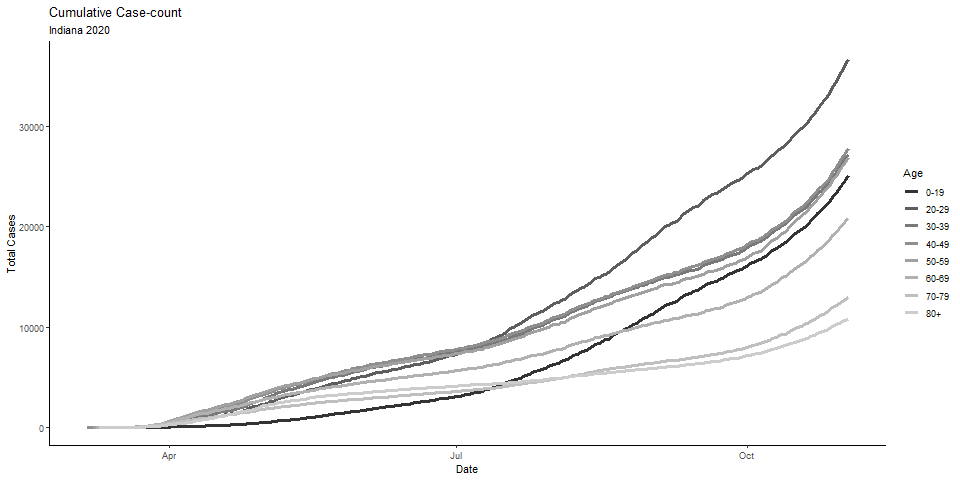
\includegraphics[width=.9\linewidth]{../figs/indianacasecounts.png}
  \caption{Indiana case-counts per day}
  \label{fig:in-cases}
\end{subfigure}
\begin{subfigure}{.45\textwidth}
  \centering
  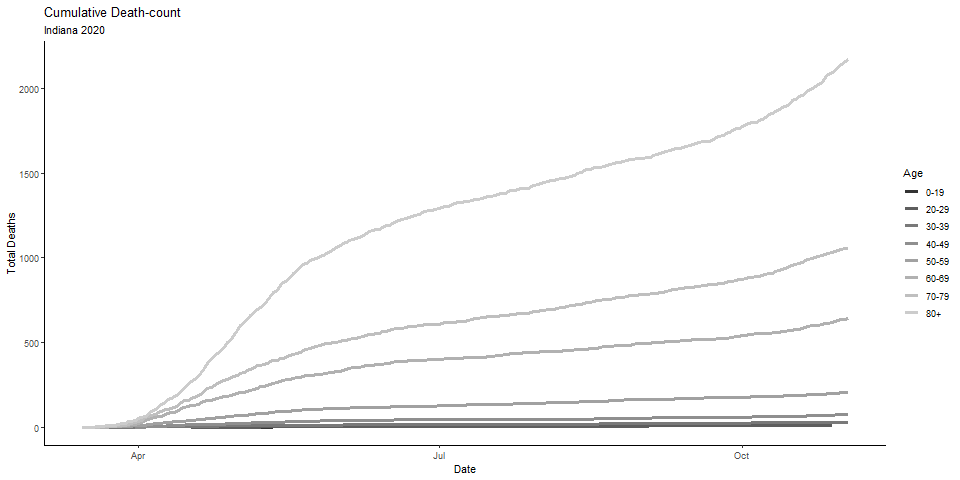
\includegraphics[width=.9\linewidth]{../figs/indianadeaths.png}
  \caption{Indiana death-counts per day}
  \label{fig:in-deaths}
\end{subfigure}
\end{figure}

\item {\bf Random/Nonrandom statewide sample}: Table~\ref{tab:indiana} summarizes data from a random sample from April 25--29th as well as a nonrandom sample obtained between May 2--3 in racial/ethnic minority communities (cite). The nonrandom sample is not a random subsample of the overall case-counts; however, this data provides important supplementary covariate information.  Namely, the samples collected included covariate information on (1) prior symptoms, (2) COVID-19 positive individual in household, and (3) prior COVID-19 positive test. To account for the nonrandom sample being from high risk areas, we adjust estimates to match the statewide positivity rate of 11.7\% between May 1--2. These adjusted rates are presented in parentheses in Table~\ref{tab:indiana}.


\begin{table}[th]
\begin{tabular}{c | c | r r | r | r r }
& & \multicolumn{2}{c}{Total Tests (\%)} & US & \multicolumn{2}{c}{Positive Test Rate (\%)}\\
\cline{3-4} \cline{6-7}
& & NonRandom & Random & Census & NonRandom & Random \\ \hline
\multirow{2}{*}{Sex} & Female & 58.2 & 55.0 & 50.7 & 21.7 (11.2) & 1.4 \\
& Male & 41.8 & 45.0 & 49.3 & 24.2 (12.4) & 2.1 \\ \hline
\multirow{3}{*}{Age} & $<40$ & 39.4 & 28.0 & 52.7 & 29.7 (15.0) & 1.7 \\
& $40-59$ & 41.1 & 36.0 & 25.2 & 24.9 (12.5) & 2.1 \\
& $\geq 60$ & 19.5 & 36.0 & 22 & 6.7 (3.4) & 0.9 \\ \hline
\multirow{2}{*}{Race} & White & 23.1 & 92.0 & 86.9 & 19.5 (9.6) & 1.5 \\
& Nonwhite & 76.9 & 8.0 & 13.1 & 25.0 (12.3) & 3.4 \\ \hline
% Hispanic & Hispanic & 44.1 & 2.0 & 7.1 & 37.6 & 6.9 \\
% Origin & Non-Hispanic & 55.9 & 98.0 & 92.9 & 13.0 & 1.3 \\ \hline
\multirow{2}{*}{Fever} & Yes & 17.0 & 1.8 & - & 66.4 (32.1) & 4.5 \\
& No & 83.0 & 98.2 & - & 15.6 (7.5) & 1.3 \\ \hline
Household & Yes & 10.8 & 1.4 & - & 46.1 & 29.4 \\
$+$ Case & No & 89.2 & 98.6 & - & 21.6 & 1.3 \\ \hline
Prior $+$ & Yes & 6.1 & 1.4 & - & 39.2 & 24.4 \\
Test & No & 93.9 & 98.6 & - & 21.6 & 1.3 \\ \hline
\end{tabular}
\caption{Estimated point prevalence of active infection with SARS-CoV-2 by demographics in Indiana.}
\label{tab:indiana}
\end{table}

\item {\bf Facebook symptom survey}: We extract daily symptom surveys completed by individuals on Facebook who identify as living in Indiana.  We collect age, sex, and demographic information as well as COVID-19 related symptoms, which Facebook defines as having (1) a fever and cough, (2) shortness of breath, \emph{or} (3) difficulty breathing. To assess potential bias, we compare the random sample from Indiana to the Facebook symptom survey data collected from April 20th to April 25th.  Table~\ref{tab:comparison} demonstrates minimal bias in the Facebook symptom survey.
\begin{table}
\centering
\begin{tabular}{c | c c c | c}
& \multicolumn{3}{c}{Facebook} & Random \\ \cline{2-5}
& Lower CI & Estimate & Upper CI & Estimate \\ \hline
Fever &  0.017 & 0.020 & 0.024 & 0.018 \\
Cough &  0.142 & 0.148 & 0.154 & 0.149 \\
Shortness & 0.058 & 0.060 & 0.062 & 0.062 \\ \hline
\end{tabular}
\caption{Comparison of Facebook symptom survey and random sample demonstrates minimal bias.}
\label{tab:comparison}
\end{table}

% \item {\bf Hospitalization data}: On each day, we observe the number of individuals who are COVID-19 positive that visited a hospital on that day.  Unfortunately, hospitalization data is not broken out by age, gender, and racial demographic information.  Instead, we rely on combining Facebook data to calculate the fraction of those who sought the hospital per week in each strata. We then use this to figure out how many individuals per strata were hospitalized and then back out how many

\item {\bf Death data}: On each day, we observe the number of deaths due to COVID-19 reported on that day, with deaths broken out jointly by age, gender, and racial demographic information.  Figure~\ref{fig:in-deaths} plots the cumulative number of COVID-19 related deaths over time by age group.
\end{itemize}


\subsection{Inverse-probability weighting approach}

We start with using Table~\ref{tab:indiana} to compute IPW weights.  The random sample is $n=3,658$.  Here, we demonstrate how to compute the weight for a particular strata.  For example, the strata defined as Male, 40--59, White, has a Fever, no household cases, and no prior tests has a weight proportional to
$$
\frac{\left( 0.493 \times 0.252 \times 0.869 \times 0.018 \right)}{\left(0.418 \times 0.411 \times 0.231 \times 0.17 \right)} = 0.628
$$
Using the constructed weights and the adjusted strata-level prevalence estimates, the IPW estimate under no measurement-error is $7.7$, a decrease of four percentage points from the observed prevalence of $11.7$. Using Table~\ref{tab:indiana} to compute weights requires the assumption of independence among factors.  To alleviate this, we compute weights using Facebook's survey data collected in Indiana over that window of time; the resulting IPW estimate under no measurement-error is

The study did not report sensitivity and specificity; therefore, we take the suggested measures from~\cite{Woloshin2020} which report 70\% sensitivity is a reasonable estimates and~\cite{Cohen2020} which report 97.6\% specificity.  This corresponds to a false negative rate of $30\%$ and false positive rate of $2.4\%$.  Therefore, the IPW estimate accounting for measurement-error is $7.7\%$.  To account for uncertainty in

Indiana's population as of 2019 was $6.732$ million.  Subtracting off the $617,555$ tests that had already performed yields a sampling fraction of $f = 0.001$.  The smoothed prevalence estimate is 28.4\%.  Adjusting for imperfect testing yields an estimate of $33.9\%$.



For this estimate, we consider estimation of data quality $E_{\I} \left[ \rho_{\tilde I(X),Y} \right]$. In \cite{Meng2018}, estimation relied on observing the true outcome (i.e., election vote totals), which is not possible in the current crisis.  Here, we use the random sample as a noisy but unbiased estimate of the true prevalence. Our goal is not inferential. Instead, we aim to build sensitivity analyses that can aid in understanding the amount of information in observational COVID case-count data.


Under the assumption that the survey is a SRS from New York, the error is $17.6$\%.  Using~\eqref{eq:error}, we construct an estimate of the relative sampling rate as follows
\[
\rho D_M = \sqrt{\frac{f}{1-f}} \frac{\text{0.176}}{\sigma_Y} = 1.07 \times 10^{-2} \Rightarrow \Delta = 1.07 \times 10^{-3} \Rightarrow M = 2.3.
\]
We can perform a sensitivity analysis by considering the range of false negative and positive rates from~\cite{Bendavid2020}, which leads to a range for $M$ of $(2.21, 2.38)$.  Therefore, the impact on bias of $\hat R_t$ appears moderate.  If $FP = 0.05$ and $FN = 0.005$, then the relative sampling rate increases to $M=3.04$.  This simple tool helps us understand how sensitivity and specificity impact biases and  therefore how much we should trust conclusions based on these assumptions.


\subsubsection{Time-varying IPW estimator}

\emph{Need to show Hospitalization C+ versus Covid count to show that most of the tests are in that subset for early parts.}






\subsection{Model-based estimation}

\subsection{Doubly robust estimation}

% \begin{figure}
% \centering
% \begin{subfigure}{.5\textwidth}
%   \centering
%   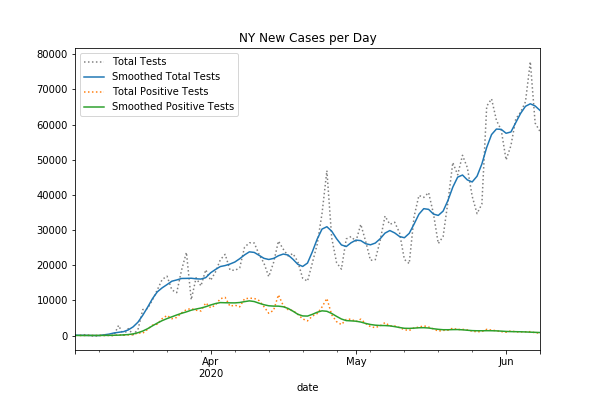
\includegraphics[width=.9\linewidth]{../methods/figs/NY_casecount.png}
%   \caption{NY new cases per day}
%   \label{fig:ny-covid-test}
% \end{subfigure}%
% \begin{subfigure}{.5\textwidth}
%   \centering
%   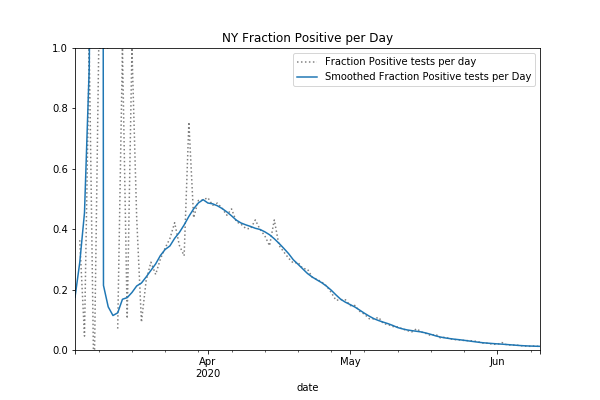
\includegraphics[width=.9\linewidth]{../methods/figs/NY_fracpos.png}
%   \caption{NY fraction of new tests positive per day}
%   \label{fig:ny-covid-frac}
% \end{subfigure}
% \caption{New York COVID-19 reported data}
% \label{fig:ny-covid}
% \end{figure}


% \section{Cross-population comparisons}
% \label{section:crosspop}
% So far we have focused on understanding the limitations of using case-count data to understand population quantities of interest for a \emph{single} population.  Many are interested in cross-population comparisons to contrast the impact of countries' mitigation policies.  Many pieces in the media as well as academic articles have plots of case-count over time aligned by time of first known case.  Others have claimed such comparisons unfair due to unequal population sizes and instead plotted case-count per million.  In this section, we focus on the statistical issues relevant to such comparisons.

% \subsection{Prevalence comparisons}

% At a fixed time, suppose prevalence estimates $\bar y_1$ and $\bar y_2$ are observed for two populations. We can express $\bar y_1 - \bar y_2$ in statistical terms as
% $$
% (\bar Y_1 - \bar Y_2) + \left[ \rho_{I_1, Y_1} \times D_{M_1} \times \sqrt{\frac{1-f_1}{f_1}} \times \sigma_{Y_1}  - \rho_{I_2, Y_2} \times D_{M_2} \times \sqrt{\frac{1-f_2}{f_2}} \times \sigma_{Y_2} \right].
% $$
% The first term is the difference in population prevalence (i.e., the quantity of interest).  If random sampling were performed in each population, $E_{\I} [ \rho_{I_j, Y_j}] = 0$ and so the estimate would be unbiased.  However, the second term represents the complex error that results from selection bias.
% The particular test of interest is $H_0: \bar Y_1 = \bar Y_2$.  Under the null, $\sigma_{Y_1} = \sigma_{Y_2}$.  In classical statistics, we would compute a Z-score:
% $$
% \begin{aligned}
% \frac{\bar y_1 - \bar y_2}{ \sqrt{V_{SRS} (\bar y_1 - \bar y_2)} } &=
% \frac{\rho_{I_1, Y_1} \times D_{M_1} \times \sqrt{\frac{1-f_1}{f_1}}  - \rho_{I_2, Y_2} \times D_{M_2} \times \sqrt{\frac{1-f_2}{f_2}} }{ \sqrt{\frac{1}{N_1 -1} \times \frac{1-f_1}{f_1} + \frac{1}{N_2 - 1} \times \frac{1-f_2}{f_2}} }  \\
% &\overset{\star}{=}
% \sqrt{\frac{(N_1-1)(N_2 -1)}{N_1 + N_2}} \left[ \rho_{I_1, Y_1} - \rho_{I_2, Y_2} \right]
% \end{aligned}
% $$
% Where the last equality holds under $f_1 = f_2$, i.e., same sampling rate relative to population size. This tells us that the exact error in the comparison of sample means, as an estimate of the difference in population means, scales as a function of the difference in data quality $\rho_{I_1, Y_1} - \rho_{I_2, Y_2}$ times a square root of a population adjustment.  For highly unequal population sizes (e.g., $N_1 \gg N_2$), the adjustment is approximated well by the square root of the smaller population size minus one (e.g. $\sqrt{N_2 -1}$).

% Take, for example, a comparison of the US and Canada.  The two population sizes are approximately 328 million and 38 million people.  Then the population adjustment is $5.84$ million. As of May 5th, Canada has performed a total of 24.92 tests per 1,000 people while the US has performed a total of 22.01 tests per 1,000 people\footnote{According to \href{https://ourworldindata.org/grapher/full-list-cumulative-total-tests-per-thousand}{ourworldindata.org}} so the data quantities are approximately equal to $f = 23/1000 = 0.023$.  Then, under a prevalence of 10\%, one would need the differential $\Delta_1-\Delta_2$ to be much smaller than $11.68 \times 10^{-6}$ in order for the selection bias to not impact.  So only under the very strong assumptions of equal data quantity and quality will the comparisons be valid and the $Z$-score can be treated as in the classical setting.  A simple alternative is to use the effective sample sizes to build more appropriate $Z$-score.  That is, setting
% $$
% Z_n = \frac{\bar y_1 - \bar y_2}{ \frac{1-f}{f} \sigma_y \sqrt{ \frac{1}{n_{1,eff} - 1} + \frac{1}{n_{2,eff} - 1}}}
% $$
% allows us to build Z-scores that account for the true sample size.  While still not perfect, this allows us to build Z-scores that are not overly confident due to selection bias and measurement error.  See Section~\ref{section:est_dq} for discussion of how to estimate data quality.

\section{Discussion}
\label{section:discussion}

{\bf Our goal with surveillance is to identify areas of weakness; but selection bias is an issue!}

There is nothing routine about COVID-19, including the corresponding statistical questions.  The goal of this paper was to point out questionable statistical routines.  Precision in reported case-count data gives the illusion of information when what what is needed is quantification of uncertainty. Selection bias leads data analysts to feel certain about incorrect conclusions.  We end with a brief discussion of important related topics.

\subsection*{Additional biases and measurement-error}

Length bias and measurement-error?

\subsection*{Decision-making: data versus information}

Having read through the above technical discussions, one may come to the incorrect conclusion that because we are concerned about implicit biases in observational data, we must wait for better data sources in order to act~\citep{Ioannidis2020}.  This conclusion confuses data and information.  Lack of high quality data means we should be skeptical regarding conclusions drawn from these data sources alone.  Being skeptical of observed data does not imply governments and communities should wait for high quality data to act; this is especially true in the current high risk scenario.  Instead, we should aim to have high quality information.  Yet in the current crisis we have just that.  Indeed, epidemiologists and public health officials have a strong understanding of the basic facts of pandemics and disease spread.  Social distancing, contact tracing and mass testing are all important.  Individuals and communities with low quality data and only basic information will hopefully make decisions that respect inherent risks to their well being as well as the high degree of uncertainty in the observed data. Of course, there are trade-offs and long-term stay-at-home orders will have negative economic consequences.  A full discussion of these topics is beyond the scope of the current article.

\subsection*{Data quantity versus quality}

Governments implicitly argue that increased testing capacity will perform the above task.  Without complete compliance, however, our understanding of future outbreaks may be plagued by self-selection bias, compounded by changing sensitivity and specificity rates. Random testing removes these effect modifiers, giving governments more information to fight the disease.  This is not to say random testing should replace current testing practices; only that the random testing should supplement and will provide valuable additional information even with moderate sample sizes.

\subsection*{High quality information on prevalence.}

Governments are pushing for increased testing capacity and robust contact tracing.  Contact tracing is incredibly useful for identifying carriers early and preventing spread of the disease.  We would argue that, after the current wave, understanding prevalence is also key.  We know that the probability of an outbreak is a function of current prevalence and network connectivity.  Epidemic critical thresholds have been derived for many infectious disease models~\citep{Pastor2001,Newman2002,Parshani2010}.  Knowing prevalence will help governments determine long-term community-level risk and allow for more targeted interventions -- shutting down only certain locations when necessary.

\subsection*{Stratified sampling: improving precision in low-prevalence environments.}
Random sampling is a powerful tool.  One difficulty with SRS is when prevalence is low.  Consider the Santa Clara study~\citep{Bendavid2020} which estimated prevalence less than 2\% in the county.  The key issue with low prevalence is that if the test's specificity is higher than the prevalence, then the observed data is consistent with zero recovered individuals. In these settings, SRS is likely to fail; however, there are potential solutions.  One can, for example, stratify the population into risk categories (e.g., based on population density, occupation, age) and perform Neyman allocation~\citep{Cochran77}.

\subsection*{Model-based solutions.}

One can extend the SIR model to account for selection bias and measurement error. Without strong assumptions on the selection mechanism, however, the estimates are often not identifiable.  When an issue ``cannot be resolved nonparametrically then it is usually dangerous to resolve it parametrically''\citep{CoxHink74}. Absent random sampling, the best route forward for all data analyses is careful associated sensitivity analyses and humility in data-driven conclusions.

\subsection*{Random sampling for doubly robust estimation}

Selection rates are likely time-varying; therefore, we need rapid survey samples to properly model the selection criteria for doubly robust inferential procedures.

COLLECT COVARIATE INFORMATION (even aggregate) and provide it in accessible formats.

- Easy access to history of testing requirements
- Smaller random samples over time (at least as testing and prevalence changes drastically) to assess selection changes
- Record symptom/asymptomatic status and COVID contact.  If not for all, then for at least some we need these covariates!!!!!

\subsection*{Systematic data collection and reporting}

I would say this is important but JHU is not enough; see above for benefits of random sampling to augment and improve decision making.

\subsection*{Frequency and turnaround time}

This supposes no selection bias.




What is your goal?  "get people who are currently sick off the street." Then test frequently and often.  But we dont live in a mandatory testing environment (nor is it currently capable).  Random testing is one way to improve upone current practice whiel we wait for that

{\bf COORDINATION ON DATA SOURCES}

\bibliographystyle{plainnat}
\bibliography{covid-refs}

\newpage
\appendix

\section{Reproducible code}

All relevant code can be found at \url{https://github.com/wdempsey/covid-umich}.

\section{Technical details}

Suppose disease prevalence was estimated as the fraction who tested positive for COVID-19, i.e., $\bar y_n^\star = \frac{\sum_{i=1}^N I_j Y_j^\star}{\sum_{i=1}^N I_j}$.  We can again investigate the error compared to the true prevalence $\bar Y$ in statistical terms:
$$
\bar y_n^\star - \bar Y = \sqrt{\frac{1-f}{f}} \left[ \rho_{I,Y} \times \sigma_Y + \rho_{I,PZ} \times \sigma_{PZ} + \sqrt{\frac{f}{1-f}}  \left( FP - (FP+FN) \bar Y \right) \right] .
$$
where $Z = 1-2Y$; see Appendix~\ref{app:imperfect} for the derivation. The first term in the large brackets represents the perfect testing regime; to this end, we refer to $\rho_{I,Y}$ as the \emph{true data quality}.  The second term represents the interaction between imperfect testing and selection bias. The variable $PZ = 1[Y=0,P=1] - 1[Y=1, P=1]$ is non-zero only when $P=1$ (i.e., the outcome is incorrectly reported) and the sign depends on the true outcome $Y$.  Given this, we refer to $\rho_{I,PZ}$ as the \emph{observed data quality} that accounts for both selection bias and measurement error.  In the appendix, we show the sign of $\rho_{I,PZ}$ is the opposite of the sign of $\rho_{I,Y}$, which implies that the observed data quality adds error in the opposite direction from the true data quality.  Finally, the third term represents the bias due to imperfect testing.

\subsubsection{Connecting true and observed data quality}

We start by considering the first two terms and assess whether the sign of the bias can reverse due to the interaction of measurement error and selection bias.  To do this, we define the sampling rates differential.  Let $f_1 := \pr (I_J = 1 \mid Y_J = 1)$ and $f_0 := \pr(I_J = 1 \mid Y_J = 0)$ be the sampling rates where $J$ is a random index defined on $\{1,\ldots, N\}$.  Then $\Delta = f_1 - f_0$ is the sampling rate differential.  Using these terms, we can re-express the first two terms as
$$
\rho_{I,Y} \times \sigma_Y + \rho_{I,PZ} \times \sigma_{PZ} =
\rho_{I,Y} \times \sigma_Y \left[ 1 - \Delta \times \frac{\bar Y}{1-\bar Y} \times \frac{FP(1-\bar Y) + FN \cdot \bar Y}{f_0 (1-\bar Y) + f_1 \bar Y} \right].
$$
final term represents the \emph{imperfect testing adjustment} which is a complex function of the sampling rate differential, the odds ratio, and the ratio of measurement error interaction with prevalence and sampling rates interaction with prevalence. Note $\sgn(\Delta) = \sgn(\rho_{I,Y})$ by equation~\ref{eq:binaryrho} in the Appendix, which implies the measurement error adjustment either shrinks the data quality measure toward zero or reverses its sign.

% While prior investigations have noted the interaction between measurement error and selection bias~\citep{Beesley2020,Beesley2019,Smeden2019}, the interaction with the sample size relative to the population, i.e., $f$, has largely been ignored.  The above statistical decomposition clarifies the importance of this quantity~$f$.  In particular, note that the statistical error also includes a bias term due to measurement error and this term increases as the sampled fraction $f$ increases. Therefore, how the first two terms interact with the final term depends on the fraction of the population sampled.  This interaction is complex, but implies that whether the estimate $\bar y^\star_n$ is an overestimate or underestimate is a complicated question due to the relation amongst these three pieces.

% Consider again the current COVID-19 pandemic. For now, we continue to assume the ratio of conditional selection rates $f_1/f_0$ is equal to 1.5.  In Section~\ref{section:est_dq}, we discuss recent research suggesting a false negative rate around 17.2\% and a false positive rate around 0.05\%. Under these rates and the current US prevalence rates, the ratio of the MSE to MSE under no measurement error is 0.436; if we switch false negative rates down to 5\% and increase the false positive rate to 5\% then the relative MSE is 2.89.  This is merely to demonstrate that in some cases we see a huge increase in MSE and in other settings we have a huge decrease in MSE.  What drives this is the false positive and negative rate interaction with prevalence and sampling rates.  Therefore, whether we are better or worse off with respect to the MSE is a very difficult question to answer.

\subsection{An improved estimator under imperfect testing}


Let $P_j$ be an indicator of measurement error, equal to $1$ when we incorrectly measure the outcome and $0$ when we observe the true outcome. We suppose this is a stochastic variable where $\pr(P_j = 1 \mid Y_j = 1) =: FN$ is the false-negative rate and $\pr(P_j = 1 \mid Y_j = 0) =: FP$ is the false-positive rate.  If individual $j$ is selected (i.e., $I_j = 1$) then the observed outcome can be written as $Y_j^{\star} = Y_j(1-P_j) + (1-Y_j) P_j$.

\subsection{Derivations for imperfect testing framework.}
\label{app:imperfect}
We start by considering the empirical mean estimator under imperfect testing,
$$
\bar y_n^\star = \frac{\sum_{j=1}^N Y_j^\star I_j}{\sum_{j=1}^N I_j} = \frac{\sum_{i=1}^N  I_j Y_j^\star }{\sum_{j=1}^N  I_j } = \frac{\sum_{i=1}^N  I_j \left[ Y_j (1-P_j) + (1-Y_j) P_j \right]}{\sum_{j=1}^N  I_j }
$$
For any set of numbers $\{ A_1, \ldots, A_N \}$ we can view it as the support of a random variable $A_J$ induced by the random index $J$ defined on $\{1,\ldots, N\}$.  When $J$ is uniformly distributed $E_J (A_J) = \sum_{j=1}^N A_j / N \equiv \bar A_N$. Then
$$
\begin{aligned}
\bar y_n^\star  - \bar Y_N &= \frac{E_J \left[ I_J \left[ Y_J (1-P_J) + (1-Y_J) P_J \right] \right]}{E_J [ I_J ] } - E_J[Y_J] \\
&= \frac{E_J \left[ I_J P_J (1-2Y_J) \right]}{E_J [ I_J ] } + \left( \frac{E_J [I_J Y_J]}{E_J [ I_J ] } - \frac{E_J[Y_J] E_J[I_J]}{E_J[I_J]} \right) \\
\end{aligned}
$$
The term in parentheses can be re-written as
$$
\begin{aligned}
\frac{E_J [I_J Y_J]- E_J[Y_J] E_J[I_J]}{E_J[I_J]} &=  \frac{E_J [I_J Y_J]- E_J[Y_J] E_J[I_J]}{\sqrt{V_J(I_J) V_J(Y_J)}} \frac{\sqrt{V_J(I_J)}}{E_J[I_J]} \times \sqrt{V_J(Y_J)} \\
&= \rho_{I,Y} \times \sqrt{\frac{(1-f)}{f}} \times \sigma_Y
\end{aligned}
$$
which agrees with Meng's (2019) decomposition. For the other term, first we define $Z_j := 1 - 2 Y_j $. Then $Z_j = 1$ if $Y_j = 0$ and $Z_j = -1$ if $Y_j = 1$. Then the term can be re-written as
$$
\begin{aligned}
\frac{E_J \left[ I_J P_J (1-2Y_J) \right]}{E_J [ I_J ] } &= \left( \frac{E_J \left[ I_J P_J Z_J \right]}{E_J [ I_J ] } -  \frac{E_J \left[ P_J Z_J \right] E_J[ I_J]}{E_J [ I_J ] } \right) +  \frac{E_J \left[ P_J Z_J \right] E_J[ I_J]}{E_J [ I_J ] } \\
\end{aligned}
$$
The term in parentheses can be re-expressed using the previous technique as:
$$
\rho_{I, PZ} \times \sqrt{\frac{1-f}{f}} \times \sigma_{PZ}
$$
where now the ``data defect'' and ``problem difficulty'' are with respect to $PZ$ rather than $Y$. The final term is equal to
$$
\begin{aligned}
E_J [P_J Z_J ] &= E_J [ E_J [ P_J Z_J \mid Y_J ] ] \\
&= \pr (P = 1 \mid Y = 0) (1-\bar Y) - \pr(P=1 \mid Y = 1) \bar Y \\
&= FP - (FP + FN) \cdot \bar Y
\end{aligned}
$$
Combining these yields:
$$
\bar y_n^\star - \bar Y = \sqrt{\frac{1-f}{f}} \left(\rho_{I,Y} \sigma_Y + \rho_{I, PZ} \sigma_{PZ} \right) + \left( FP - (FP+FN) \bar Y \right)
$$

\subsubsection{Derivation of an estimator unbiased under SRS}
\label{app:memestimator}
We see the final term is given by $FP (1-\bar Y) - FN \bar Y$ is the bias associated with using the unadjusted prevalence estimate $\bar y_n^\star$.  This motivates an adjusted estimate
$$
\tilde y_n^{(0)} = \bar y_n^\star - FP (1- \bar y_n^\star ) + FN \bar y_n^\star
= \bar y_n^\star (1 + FN + FP) - FP.
$$
Now considering the error for the adjusted estimate, $\tilde y_n^{(0)} - \bar Y$, we have
$$
\begin{aligned}
 &\bar y_n^\star (1 + FN + FP) - FP - \bar Y \\
 =&(\bar y_n^\star - \bar Y) +  (FN + FP) \bar y_n^\star - FP  \\
 =&\underbrace{\sqrt{\frac{1-f}{f}} \left[\rho_{I,Y} \sigma_Y + \rho_{I, PZ} \sigma_{PZ} \right]}_{\Psi} + (  FN + FP ) (\bar y_n^\star -  \bar Y) \\
 =& \Psi + (FN + FP) \Psi + (FN + FP) (FP - (FP+FN) \bar Y).
 \end{aligned}
$$
The final term is a (smaller) bias term and so we propose another adjusted estimator $\tilde y_n^{(1)} = \tilde y_n^{(0)} + (FN+FP)  ( (FN+FP) \bar y_n^\star - FP)$, with associated error $\tilde y_n^{(1)} - \bar Y$ given by
$$
\begin{aligned}
 &(\bar y_n^{(0)} - \bar Y) + (FN+FP)  ( (FN+FP) \bar y_n^\star - FP)\\
 =&\Psi + (FN + FP) \Psi + (FN + FP) (FP - (FP+FN) \bar Y) + (FN + FP) ((FP+FN) \bar y_n^\star - FP)  \\
  =& \Psi + (FN + FP) \Psi + (FN + FP)^2 \Psi + (FN+FP)^2 (FP - (FP+FN) \bar Y).
 \end{aligned}
$$
This motivates recursively defining estimators $\tilde y_n^{(t)} = \tilde y_n^{(t-1)} + (FN+FP)  ( (FN+FP) \bar y_n - FP)$ for $t=1,2,\ldots$ where $\tilde y_n^{(0)} = \bar y_n^\star$.  Then
$$
\tilde y_n^{(t)} = \bar y_n^\star \sum_{s=0}^{t+1} (FP+FN)^s - FP \sum_{s=0}^{t} (FP+FN)^s
$$
and the associated error at iteration $t$ given by
$$
\Psi \sum_{s=0}^t (FN+FP)^s = \Psi \frac{1 - (FN+FP)^t}{1 - (FN+FP)}.
$$
We can then get an estimator with no residual bias term by taking the limit as $t$ goes to infinity; that is, define
$$
\tilde y_n = \lim_{t \to \infty} \tilde y_n^{(t)} = \frac{\bar y_n^\star - FP}{1 -(FN+FP)}.
$$
Then the associated error $\tilde y_n - \bar Y$ can be expressed as $\frac{\Psi}{1-(FN+FP)}$.

\subsection{Model-based derivation of the estimator.}
\label{app:modelbased}
The estimator $\tilde y$ was derived as a limit of a process that removes the residual bias term at each step.  Here we consider a model-based explanation.  Let $\theta = \pr( Y = 1)$ and $\phi = \pr( \text{test is positive})$.  Given a known false negative (FN) and false positive (FP) rates, we have
$$
\begin{aligned}
\phi &= \theta \cdot (1-FN) + (1-\theta) \cdot FP = \theta (1-FN-FP) + FP \\
\Rightarrow \theta &= \frac{\phi - FP}{1-FN-FP}.
\end{aligned}
$$
Thus, the estimator $\tilde y$ is also the appropriate estimator under a model-based approach.  While the derivation here is more straightforward, the derivation in the prior section provides a simple formula for the associated error $\tilde y_n - \bar Y$ and gives a novel connection between the empirical estimator $\bar y_n^\star$ and the adjusted estimator $\tilde y_n$ without reference to the model-based approach.

\subsection{Further simplification.}
For the binary outcome $Y$, we have $\sigma_Y = \sqrt{\bar Y (1-\bar Y)}$. Moreover,
$$
\begin{aligned}
V_J(P_J Z_J) &= E_J[(P_J Z_J)^2] - E_J[P_J] E_J[Z_J] \\
&= E_J[P_J] - E_J[P_J] (1 - 2 \bar Y) = 2 \bar Y E_J [ P_J ] \\
&= 2 \bar Y \left( FP (1-\bar Y) + FN \bar Y \right) \\
\Rightarrow \sigma_{PZ} &= \sqrt{ 2 \bar Y \left( FP (1-\bar Y) + FN \cdot  \bar Y \right) }
\end{aligned}
$$
Then the formula for the error is given by:
\begin{equation}
\label{eq:finalstep}
\sqrt{\frac{1-f}{f}} \left[\rho_{I,Y} \sqrt{\bar Y (1-\bar Y)} + \rho_{I, PZ} \sqrt{ 2 \bar Y \left( FP (1-\bar Y) + FN \cdot \bar Y \right )} \right] \times \frac{1}{1- (FN+FP)}
\end{equation}
By definition, we have
$$
\begin{aligned}
\rho_{I,PZ} &= \frac{C(I, PZ)}{\sqrt{V(PZ) V(I)}} \\
&= \frac{C(I, PZ)}{\sqrt{V(Y) V(I)}} \sqrt{\frac{V(Y)}{V(PZ)}} \\
&= \rho_{I,Y} \frac{C(I,PZ)}{C(I,Y)} \sqrt{ \frac{(1-\bar Y)}{2 ( FP (1-\bar Y) + FN \cdot \bar Y)} }
\end{aligned}
$$

$$
\begin{aligned}
C(I, PZ) &= E[ I P Z ] - E[I] E[PZ] \\
&=  [FP f_0 - (FP f_0 + FN f_1) \bar Y] - f [ FP - (FP+FN) \bar Y ] \\
&=  - FP \Delta \bar Y + FP \bar Y^2 \Delta - FN \bar Y^2 \Delta \\
&=  - \Delta \bar Y (FP \cdot (1-\bar Y) + FN \cdot \bar Y) \\
\end{aligned}
$$
where $f = f_1 \bar Y + f_0 (1-\bar Y)$ so $f_0 - f = -\Delta \bar Y$ and $f_1 - f = \Delta (1-\bar Y)$.
$$
\begin{aligned}
C(I, Y) &= E[ I Y ] - f \bar Y \\
&=  f_1 \bar Y + f_0 (1-\bar Y) - f \bar Y \\
&=  f_0 (1-\bar Y) + \Delta (1-\bar Y) \bar Y \\
&= (1-\bar Y) (f_0 + \Delta \bar Y)
\end{aligned}
$$
Combining yields
$$
\begin{aligned}
\rho_{I,PZ} &= \rho_{I,Y} \times \frac{- \Delta \bar Y (FP \cdot (1-\bar Y) + FN \cdot \bar Y) }{(1-\bar Y) (f_0 + \Delta \bar Y)} \times \sqrt{ \frac{(1-\bar Y)}{2 ( FP (1-\bar Y) + FN \cdot \bar Y)} } \\
&= - \rho_{I, Y} \times \Delta \times \sqrt{\frac{\bar Y}{1-\bar Y}} \frac{\sqrt{FP(1-\bar Y) + FN \cdot \bar Y}}{f_0 (1-\bar Y) + f_1 \bar Y} \times \sqrt{\frac{\bar Y}{2}}
\end{aligned}
$$
We can then re-write $\rho_{I,Y} \sigma_Y + \rho_{I,PZ} \sigma_{PZ}$ as
$$
\rho_{I,Y} \sigma_Y \left( 1 - \Delta \times \frac{\bar Y}{1-\bar Y} \times \frac{FP(1-\bar Y) + FN \cdot \bar Y}{f_0 (1-\bar Y) + f_1 \bar Y} \right).
$$
Inserting into equation~\eqref{eq:finalstep} yields the desired result.

\subsection{Derivation of effective sample size}
\label{app:effss}

Let $S_Y^2 = (N-1)^{-1} \sum_{j=1}^N (Y_j - \bar Y)^2$ be the population variance as defined in survey sampling~\citep{Cochran77}.  Then $\sigma_Y^2 = (N-1)/N \cdot S_Y^2$.  Under SRS, the MSE is the variance as the estimate is unbiased and the variance is given by $(1-f)/n S_Y^2$.  Then setting the MSE under general selection and SRS equal we have
$$
\begin{aligned}
\underbrace{\frac{1-f}{f} \times E_{\I} \left[ \rho_{I, Y}^2 \times D_M^2 \right]}_{1/n_{eff}^\star} \times \sigma_Y^2 &= \frac{1-f}{n_{eff}} S_Y^2 \\
\frac{1}{n_{eff}^\star} \times \frac{N-1}{N} S_Y^2 &= \frac{1-f}{n_{eff}} S_Y^2 \\
\frac{1}{n_{eff}^\star} &=  \left( \frac{1}{n_{eff}} - \frac{1}{N} \right) \left( \frac{N}{N-1} \right) \\
\frac{1}{n_{eff}^\star} \left[ 1 - \frac{1}{N} + \frac{n_{eff}^\star}{N} \right]  &=  \frac{1}{n_{eff}} \\
n_{eff}^\star \left[ 1 - \frac{1}{N} + \frac{n_{eff}^\star}{N} \right]^{-1}  &=  n_{eff} \\
\frac{n_{eff}^\star}{ 1 + (n_{eff}^\star -1) N^{-1}} &=  n_{eff} \\
\end{aligned}
$$
Then if $n_{eff}^\star \geq 1$, we have that
$$
n_{eff} \leq n_{eff}^\star = \frac{f}{1-f} \times \frac{1}{E_{\I} \left[ \rho^2_{I, Y} \times D_M^2 \right]}
$$

\subsection{Ratio estimator}
\label{app:ratio}

Let ${\bf u} = (u_{t-1},u_t) \in \mathbb{R}^2$ and $g({\bf u}) = \frac{u_t}{u_{t-1}}$, i.e., a differentiable function $g:\mathbb{R}^2 \to \mathbb{R}$. Centering a Taylor series expansion of second-order around coordinates $(U_2, U_1) \in \mathbb{R}^2$ yields
$$
\begin{aligned}
g({\bf u}) =& g(U_{t-1}, U_t) - \frac{U_t}{U_{t-1}^2} (u_{t-1} - U_{t-1}) + \frac{1}{U_{t-1}} (u_t - U_t) \\
&+ \frac{1}{2} \left[ \frac{2 U_t}{U_{t-1}^3} (u_{t-1} - U_{t-1})^2 + 0 \times (u_t - U_t)^2 - 2 \times (u_{t-1} - U_{t-1}) (u_t - U_t) \frac{1}{U_t^2} \right]
\end{aligned}
$$
Plugging in $(\bar y_{t-1}, \bar y_t)$ for $(u_{t-1}, u_t)$ and $(\bar Y_{t-1}, \bar Y_t)$ for $(U_{t-1}, U_t)$ yields the $\frac{\bar y_t}{\bar y_{t-1}} - \frac{\bar Y_t}{\bar Y_{t-1}} $ is equal to
$$
\begin{aligned}
=&
- \frac{\bar Y_t}{\bar Y_{t-1}^2} (\bar y_{t-1} - \bar Y_{t-1}) + \frac{1}{\bar Y_{t-1}} (\bar y_t - \bar Y_t) \\
&+ \frac{\bar Y_t}{\bar Y_{t-1}^3} (\bar y_{t-1} - \bar Y_{t-1})^2 -  (\bar y_{t-1} - \bar Y_{t-1}) (\bar y_t - \bar Y_t) \frac{1}{\bar Y_{t-1}^2} \\
&= \frac{\bar Y_t}{\bar Y_{t-1}} \bigg[  \rho_{I_t,Y_t} \sqrt{\frac{1-f_t}{f_t}} CV (Y_t)  -\rho_{I_{t-1},Y_{t-1}} \sqrt{\frac{1-f_{t-1}}{f_{t-1}}} CV (Y_{t-1}) \\
&+ \rho^2_{I_{t-1},Y_{t-1}} \frac{1-f_{t-1}}{f_{t-1}} CV^2 (Y_{t-1}) -  \rho_{I_{t-1},Y_{t-1}} \sqrt{\frac{1-f_{t-1}}{f_{t-1}}} CV (Y_{t-1}) \times
\rho_{I_t,Y_t} \sqrt{\frac{1-f_t}{f_t}} CV (Y_t)   \bigg] \\
&= \frac{\bar Y_t}{\bar Y_{t-1}} \bigg[ \rho_{I_t,Y_t} \sqrt{\frac{1-f_t}{f_t}} CV (Y_t)  -\rho_{I_{t-1},Y_{t-1}} \sqrt{\frac{1-f_{t-1}}{f_{t-1}}} CV (Y_{t-1}) \bigg] \left[ 1 - \rho_{I_{t-1},Y_{t-1}} \sqrt{\frac{1-f_{t-1}}{f_{t-1}}} CV (Y_{t-1}) \right]
\end{aligned}
$$
where the second equality is obtained by plugging in the statistical decomposition of the error for both time points and the coefficient of variation being defined as $CV(Y) := \sigma_Y/\mu_Y$.  Under measurement error, the extra terms $D_{t}$ and $D_{t-1}$ can be inserted in the correct locations.

\subsection{Estimation of effective reproduction number}

Let
$$
\delta_t := \bigg[ \rho_{I_t,K_t} D_{M_t} \sqrt{\frac{1-f_t}{f_t}} CV (K_t)  -\rho_{I_{t-1},K_{t-1}} D_{M_{t-1}} \sqrt{\frac{1-f_t}{f_t}} CV (K_{t-1}) \bigg].
$$
Then the previous sections derivation shows that the estimate of the number of new cases on day t is given by
$$
\frac{S_t \cdot \bar y_t}{S_{t-1} \cdot \bar y_{t-1}} =
\frac{K_t}{K_{t-1}} \left( 1 + \delta_t \times \left[ 1 - \rho_{I_{t-1},K_{t-1}} D_{M_{t-1}} \sqrt{\frac{1-f_t}{f_t}} CV (K_{t-1}) \right] \right)
$$
Then setting $e_t = \delta_t \times [1 - \rho_{I_{t-1},K_{t-1}} D_{M_{t-1}} \sqrt{\frac{1-f_t}{f_t}} CV (K_{t-1}) ]$, we have
$$
\begin{aligned}
\log \left( \frac{S_t \bar y_t}{S_{t-1} \bar y_{t-1}} \right) - \log \left( \frac{K_t}{K_{t-1}} \right) &= \log (1 + e_t) \\
\log \left( \frac{\bar y_t}{\bar y_{t-1}} \right) - \log \left( \frac{K_t}{K_{t-1}} \right) &= 1 + e_t - \log \left( \frac{S_t}{S_{t-1}} \right) \\
1 + \frac{1}{\gamma} \log \left( \frac{\bar y_t}{\bar y_{t-1}} \right) - \left[ 1 + \frac{1}{\gamma} \log \left( \frac{K_t}{K_{t-1}} \right) \right] &= \frac{1}{\gamma} \left[ \log \left( 1 + e_t \right) - \log \left( \frac{S_{t}}{S_{t-1}} \right) \right] \\
\Rightarrow \hat R_t - R_t &= \frac{1}{\gamma} \left[ \log \left( 1 + e_t \right) - \log \left( \frac{S_{t}}{S_{t-1}} \right) \right]
\end{aligned}
$$

\subsection{Computating the effective sample size}
\label{section:effss}

For binary outcomes, we have
\begin{equation} \label{eq:binaryrho}
\rho_{I,Y} = \Delta \sqrt{\frac{\bar Y (1 - \bar Y)}{f (1-f)} }
\end{equation}
where $\Delta = P_J (I_J = 1 \mid Y_J = 1) - P(I_J = 1 \mid Y_J = 0) = f_1 - f_0$.  Suppose that $M = f_1/f_0$; then $f_0 = f / (\bar Y \cdot (M-1) + 1)$.  Using the upper bound $E_{\I} [ \rho_{I,Y}^2 ] \leq E_{\I} [\rho_{I,Y} ]^2$, we compute effective sample size under a range of values $\bary$, $M$ with $f = 0.066$ (i.e., current sampling fraction) and observed prevalence $0.095$.

\begin{table}[ht]
\centering
\begin{tabular}{rrrrrr}
& \multicolumn{5}{c}{$M$} \\ \cline{2-6}
$\bar y$ & 1.2 & 1.4 & 1.6 & 1.8 & 2 \\
  \hline
0.05 & 11303 & 2882 & 1306 & 749 & 489 \\
  0.07 & 6065 & 1558 & 712 & 411 & 270 \\
  0.09 & 3862 & 1000 & 460 & 268 & 177 \\
  0.11 & 2724 & 711 & 329 & 193 & 129 \\
  0.13 & 2057 & 541 & 252 & 149 & 100 \\
   \hline
\end{tabular}
\end{table}

We also present the same plot under $FP = 0.005$ and $FN = 0.172$ to show the impact of measurement error on effective sample size.

\begin{table}[ht]
\centering
\begin{tabular}{rrrrrr}
& \multicolumn{5}{c}{$M$} \\ \cline{2-6}
$\bar y$ & 1.2 & 1.4 & 1.6 & 1.8 & 2 \\
  \hline
0.05 & 6480 & 1656 & 752 & 432 & 282 \\
  0.07 & 3304 & 852 & 391 & 227 & 149 \\
  0.09 & 2059 & 536 & 248 & 145 & 97 \\
  0.11 & 1440 & 379 & 177 & 104 & 70 \\
  0.13 & 1086 & 288 & 136 & 81 & 55 \\
   \hline
\end{tabular}
\end{table}

\section{Effect modifiers in COVID-19 clinical trials}

Here we show how selection bias and measurement error can creep into clinical trial analysis. The key concern is whether clinical trials on COVID-19 recruit from the pool of individuals who have tested positive for COVID-19 or whether they sample randomly from the population, test, and then recruit from this subset of tested individuals.  To see this issue, suppose we have an outcome $Y$, a treatment $A$ and an \emph{unobserved} variable $U$.  Suppose treatment is assigned at random, i.e., $A =1$ with probability $50\%$ and $A=0$ with probability $50\%$.  Suppose the conditional mean of the outcome satisfies  $E(Y \mid U, A ) = \beta_0 + \beta_1 A + \beta_2 U + \beta_3 A U$.  Typically, we are interested in the \emph{causal effect} of $A$ on $Y$.  In counterfactual language,
$$
E( Y(A=1) - Y(A=0) ) = E_U ( E_A ( Y(A=1) - Y(A=0) \mid U=u ))
= \beta_1 + \beta_3 E(U).
$$
Even in a randomized experiment, the question is what the correct value for $E(U)$ is. For COVID-19, the value of interest is likely the expected value of $U$ in the population of COVID-19 positive individuals, i.e., $E_J [ U_J Y_J]/ E_J[Y_J] = \sum_{j=1}^N U_j Y_j / \sum_{j=1}^N Y_j$.  Assuming no measurement error, the estimator is given by the ratio $\sum_{j=1}^n y_i u_i / \sum_{j=1} y_i$.  Due to selection bias, the bias in the marginal treatment effect compared to the true marginal effect of interest is approximately equal to
$$
\beta_3 \times \sqrt{\frac{1-f}{f}} \times \frac{\bar U^\prime}{\bar Y} \bigg[ \rho_{I,U^\prime} \times CV (U^\prime)  - \rho_{I,Y} \times CV (Y) \bigg] \left[ 1 - \rho_{I,Y} \sqrt{\frac{1-f}{f}} CV (Y) \right]
$$
where $U^\prime = U Y$.  The derivation again uses a second-order Taylor series approximation and follows exactly the same as in Appendix~\ref{app:ratio}. Selection bias then leads to the estimated effect being biased if $\beta_1 \neq 0$.  Directionality of the bias will depend on the relationship between $U$ and $Y$.  If $U$ is a measure of disease severity, then it could be expected to see $\beta_3 > 0$ and $\rho_{I,U^\prime} \times CV (U^\prime)  > \rho_{I,Y} CV (Y)$.  In such situations, the treatment effect estimates will tend to be overly optimistic as most individuals recruited are potentially higher on the severity index than the population average.  Not only that, but for fixed data quality, the error compared to SRS in terms of effect estimation scales with the population size (i.e., the law of large populations).

Randomization of treatment assignment in clinical trials negates unobserved confounders.  This, however, does not negate effect modifiers.  Therefore, for marginal treatment effects to be interpretable, there must be a well-defined population.  Most often, our main interest is in causal effects on the population of COVID-19 positive.  Randomization within the clinical trial design yields internal validity, but we also need external validity to estimate the correct marginal effect of interest~\citep{Keiding2016}.

\section{IPW statistical error decomposition derivation}
\label{app:ipwderivation}
We start by considering the empirical weighted mean estimator under imperfect testing,
$$
\bar y_n^\star = \frac{\sum_{j=1}^N W_j Y_j^\star I_j}{\sum_{j=1}^N W_j I_j} = \frac{\sum_{i=1}^N  I_j W_j Y_j^\star }{\sum_{j=1}^N  I_j } = \frac{\sum_{i=1}^N  I_j \left[ Y_j (1-P_j) + (1-Y_j) P_j \right]}{\sum_{j=1}^N  I_j }
$$
Then
$$
\begin{aligned}
\bar y_n^\star  - \bar Y_N &= \frac{E_J \left[ I_J W_J \left[ Y_J (1-P_J) + (1-Y_J) P_J \right] \right]}{E_J [ I_J W_J ] } - E_J[Y_J] \\
&= \frac{E_J \left[ I_J W_J P_J (1-2Y_J) \right]}{E_J [ I_J W_J ] } + \left( \frac{E_J [I_J W_J Y_J]}{E_J [ I_J W_J ] } - \frac{E_J[Y_J] E_J[I_J W_J]}{E_J[I_J W_J]} \right) \\
\end{aligned}
$$
The term in parentheses can be re-written as
$$
\begin{aligned}
\frac{E_J [I_J W_J Y_J]- E_J[Y_J] E_J[I_J W_J]}{E_J[I_J W_J]} &=  \frac{E_J [I_J W_J Y_J]- E_J[Y_J] E_J[I_J W_J]}{\sqrt{V_J(I_J W_J) V_J(Y_J)}} \frac{\sqrt{V_J(I_J W_J)}}{E_J[I_J]} \times \sqrt{V_J(Y_J)} \\
&= \rho_{\tilde I (X),Y} \times \frac{\sqrt{V_J(I_J W_J)}}{E_J[I_J]} \times \sigma_Y
\end{aligned}
$$
Then
\begin{align*}
E_J (I_J W_J) &= P(I_J = 1) E_J [W_J \mid I_J = 1] = f \times E_J [W_J \mid I_J = 1] \\
V_J(I_J W_J) &= E[ I_J W_J^2] - E[I_J W_J]^2 \\
&= f \cdot \left( E [W_J^2 \mid I_J = 1] - f E[W_J \mid I_J = 1 ]^2 \right) \\
&= f \cdot \left( E [W_J^2 \mid I_J = 1] \pm E[W_J \mid I_j = 1]^2 - f E[W_J \mid I_J = 1 ]^2 \right) \\
&= f \cdot \left( V (W_J \mid I_J = 1) + E[W_J \mid I_J = 1]^2 (1-f) \right)
\end{align*}
Taking the ratio:
$$
\sqrt{\frac{f \cdot \left( V (W_J \mid I_J = 1) + E[W_J \mid I_J = 1]^2 (1-f) \right)}{f^2 E_J [W_J \mid I_J = 1]^2}} = \sqrt{\frac{1 - f + CV(W)^2}{f}}
$$
which agrees with Meng's (2019) decomposition of weighted outcome. For the other term, first we define $Z_j := 1 - 2 Y_j $. Then $Z_j = 1$ if $Y_j = 0$ and $Z_j = -1$ if $Y_j = 1$. Then the term can be re-written as
$$
\begin{aligned}
\frac{E_J \left[ I_J W_J P_J (1-2Y_J) \right]}{E_J [ I_J W_J ] } &= \left( \frac{E_J \left[ I_J W_J P_J Z_J \right]}{E_J [ I_J W_J ] } -  \frac{E_J \left[ P_J Z_J \right] E_J[ I_J W_J]}{E_J [ I_J W_J ] } \right) +  \frac{E_J \left[ P_J Z_J \right] E_J[ I_J W_J]}{E_J [ I_J W_J ] } \\
\end{aligned}
$$
The term in parentheses can be re-expressed using the previous technique as:
$$
\rho_{\tilde I, PZ} \times \sqrt{\frac{1-f+CV(W)^2}{f}} \times \sigma_{PZ}
$$
where now the ``data defect'' and ``problem difficulty'' are with respect to $PZ$ rather than $Y$. The final term is equal to
$$
\begin{aligned}
E_J [P_J Z_J ] &= E_J [ E_J [ P_J Z_J \mid Y_J ] ] \\
&= \pr (P = 1 \mid Y = 0) (1-\bar Y) - \pr(P=1 \mid Y = 1) \bar Y \\
&= FP - (FP + FN) \cdot \bar Y
\end{aligned}
$$
Combining these yields:
$$
\bar y_n^\star - \bar Y = \sqrt{\frac{1-f+CV(W)^2}{f}} \left(\rho_{\tilde I(X),Y} \sigma_Y + \rho_{\tilde I(X), PZ} \sigma_{PZ} \right) + \left( FP - (FP+FN) \bar Y \right)
$$
By previous arguments, we have
$$
\rho_{\tilde I (X), PZ} = \rho_{\tilde I(X), Y} \times \frac{C(\tilde I(X), PZ)}{C(\tilde I(X), Y)} \sqrt{ \frac{1-\bar Y}{ 2 (FP(1-\bar Y) + FN \bar Y)} }
$$
Then
\begin{align*}
C(IW, PZ) &= E[IWPZ] - E[IW] E[PZ] \\
&=  [FP \tilde f_0  - (FP \tilde f_0 + FN \tilde f_1) \bar Y]  - \tilde f \cdot ( FP - (FP+FN) \bar Y )\\
&= -FP \tilde \Delta \bar Y + FP \bar Y^2 \Delta - FN \bar Y^2 \Delta \\
&= -\tilde \Delta \bar Y ( FP \cdot (1-\bar Y) + FN \cdot \bar Y)
\end{align*}
where $\tilde f_i = E[ I_J W_J \mid Y_J = i]$ for $i \in \{0,1 \}$ and $f = \tilde f_1 \bar Y + \tilde f_0 (1-\bar Y)$. Moreover,
\begin{align*}
C(\tilde I,Y) &= E[ I W Y ] - \tilde f \bar Y \\
&= \tilde f_1 \bar Y + \tilde f_0 (1-\bar Y) - \tilde f \bar Y \\
&= \tilde f_0 (1-\bar Y) + \tilde \Delta (1-\bar Y) \bar Y \\
&= (1- \bar Y) (\tilde f_0 + \tilde \Delta \bar Y)
\end{align*}
Combining yields
$$
\begin{aligned}
\rho_{\tilde I (X),PZ} &= \rho_{\tilde I(X),Y} \times \frac{- \tilde \Delta \bar Y (FP \cdot (1-\bar Y) + FN \cdot \bar Y) }{(1-\bar Y) (\tilde f_0 + \tilde \Delta \bar Y)} \times \sqrt{ \frac{(1-\bar Y)}{2 ( FP (1-\bar Y) + FN \cdot \bar Y)} } \\
&= - \rho_{\tilde I(X), Y} \times \Delta \times \sqrt{\frac{\bar Y}{1-\bar Y}} \frac{\sqrt{FP(1-\bar Y) + FN \cdot \bar Y}}{\tilde f_0 (1-\bar Y) + \tilde f_1 \bar Y} \times \sqrt{\frac{\bar Y}{2}}
\end{aligned}
$$
We can then re-write $\rho_{\tilde I (X),Y} \sigma_Y + \rho_{\tilde I(X),PZ} \sigma_{PZ}$ as
$$
\rho_{\tilde I(X),Y} \sigma_Y \left( 1 - \tilde \Delta \times \frac{\bar Y}{1-\bar Y} \times \frac{FP(1-\bar Y) + FN \cdot \bar Y}{\tilde f_0 (1-\bar Y) + \tilde f_1 \bar Y} \right).
$$
Thus yielding the desired result.

\section{Doubly robust statistical error decomposition derivation}
\label{app:DRderivation}
We start by considering the empirical weighted mean estimator under imperfect testing,
\begin{align*}
&\frac{1}{N} \sum_{j=1}^N \mu(X_j) - \frac{\sum_{j=1}^N I_j W_j \mu(X_j)}{\sum_{j=1}^N I_j W_j} + \frac{\sum_{j=1}^N I_j W_j Y_j^\star}{\sum_{j=1}^N I_j W_j} \\
=& \frac{\sum_{i=1}^N  I_j W_j \left( \left[ Y_j (1-P_j) + (1-Y_j) P_j \right] - \mu (X_j) \right)}{\sum_{j=1}^N  I_j W_j } + \frac{1}{N} \sum_{j=1}^N \mu(X_j
)
\end{align*}
Then
$$
\begin{aligned}
&\frac{E_J \left[ I_J W_J \left( \left[ Y_J (1-P_J) + (1-Y_J) P_J \right] - \mu(X_J) \right) \right]}{E_J [ I_J W_J ] } - E_J[Y_J -\mu (X_J)] \\
= &\frac{E_J \left[ I_J W_J P_J (1-2Y_J) \right]}{E_J [ I_J W_J ] } + \left( \frac{E_J [I_J W_J (Y_J -\mu (X_J))]}{E_J [ I_J W_J ] } - \frac{E_J[Y_J-\mu(X_J)] E_J[I_J W_J]}{E_J[I_J W_J]} \right) \\
\end{aligned}
$$
The term in parentheses can be re-written as
$$
\begin{aligned}
&\frac{E_J [I_J W_J (Y_J-\mu(X_J))]- E_J[(Y_J-\mu(X_J))] E_J[I_J W_J]}{E_J[I_J W_J]} \\
=  &\frac{E_J [I_J W_J (Y_J-\mu(X_J))]- E_J[(Y_J-\mu(X_J))] E_J[I_J W_J]}{\sqrt{V_J(I_J W_J) V_J(Y_J-\mu(X_J))}} \frac{\sqrt{V_J(I_J W_J)}}{E_J[I_J]} \times \sqrt{V_J(Y_J-\mu(X_J))} \\
= &\rho_{\tilde I (X),Y-\mu(X)} \times \frac{\sqrt{V_J(I_J W_J)}}{E_J[I_J]} \times \sigma_{Y-\mu(X)}
\end{aligned}
$$
From prior derivations, we then have the desired result.

\section{Asymptotic derivations}
\label{app:asympderivations}

% https://www.thelancet.com/journals/lanres/article/PIIS2213-2600%2820%2930453-7/fulltext
% https://www.medrxiv.org/content/10.1101/2020.04.26.20080911v1.full.pdf

Based on~\cite{Woloshin2020}, we set the false positive rate to 2.4\% and false negative rate to 17.5\%.  To allow for potential uncertainty, we assume two \emph{synthetic} simple random samples.  The first is a simple random sample of true negative cases denoted $S_{FP}$; the second is simple random sample of true positive cases denoted $S_{FN}$.  As $\mu_t$ and $\theta_{t}$ are estimated independently at each time $t$, we can focus on the estimating equations per time point separately.  The estimates are given by:
$$
\left (
\begin{array}{c}
\frac{1}{N} \sum_{j=1}^N I_{j,t} \frac{Y_{j,t} - (1-FP-FN) \cdot (\mu_t+FP)}{\pi_{j,t}} \\
\frac{1}{N} \sum_{t^\prime = 1}^T K_{t,t^\prime} \sum_{j=1}^N I_{j,t^\prime} X_{j,t^\prime} - \frac{1}{N} \sum_{j = 1}^N \tilde I_{j,t^\prime} \tilde W_{j,t^\prime}  \pi_{j,t^\prime} X_{j,t^\prime}  \\
\frac{1}{n_{FP}} \sum_{j \in S_{FP}} \frac{Z_j}{FP} - \frac{1-Z_j}{1-FP} \\
\frac{1}{n_{FN}} \sum_{j \in S_{FN}} \frac{\tilde Z_j}{FN} - \frac{1-\tilde Z_j}{1-FN} \\
\end{array}
\right ) = {\bf 0}
$$
where $\pi_{j,t^\prime} = \pi (X_{j,t^\prime}; \theta_t)$, $Z_j$ is an indicator of a false positive in the sample $S_{FP}$  and $\tilde Z_j$ is an indicator of a false negative in the sample $S_{FN}$.  We assume the synthetic $|S_{FP}|^{-1} \sum_{j \in S_{FP}} Z_j = 0.024$ and $|S_{FP}|^{-1} \sum_{j \in S_{FP}} Z_j = 0.175$.  Sample sizes, denoted $n_{FP}$ and $n_{FN}$ respectively, are chosen to achieve desired estimator variance: $1.96/0.155^2 \cdot \sqrt{0.175 \cdot (1-0.175)} = 31$.

Under joint randomization of propensity score model and sampling designs, we have $E [ \Phi_n (\eta) ] = {\bf 0}$.  Consistency then follows by arguments in Section 3.2 of Tsiatis (2006). Under conditions C1-C6 from~\cite{Chen2019} and the additional assumption that $h_n \to 0$ as the sample size per timepoint of the sample size grows, we have $\Phi_n (\hat \eta) = 0$ and $\Phi_n (\eta_0) = O_p ( \tilde n^{-1/2} )$.  By a first-order Taylor expansion we have $\hat \eta - \eta_0 = \left[ \right]^{-1} \Phi_n(\eta_0) + o_p (\tilde n^{-1/2})$ where $\phi_n(\eta) = \partial \Phi_n (\eta)/\partial \eta$.  To calculate
$$
\frac{\partial \Phi (\eta)}{\partial \mu_t} =
\left (
\begin{array}{c}
-\frac{(1-FP-FN)}{N} \sum_{j=1}^N \frac{I_{j,t}}{\pi_{j,t}} \\
0 \\
0 \\
0
\end{array}
\right )
$$

$$
\frac{\partial \Phi (\eta)}{\partial \theta_t} =
\left (
\begin{array}{c}
-\frac{1}{N} \sum_{j=1}^N I_{j,t} (Y_{j,t} - (1-FP-FN) \cdot (\mu_t + FP)) \frac{1-\pi_{j,t}}{\pi_{j,t}} X_{j,t}^\top \\
- \frac{1}{N} \sum_{t^\prime = 1}^T K_{t,t^\prime} \sum_{j = 1}^N \tilde I_{j,t^\prime} \tilde W_{j,t^\prime}  \pi_{j,t^\prime} (1-\pi_{j,t^\prime}) X_{j,t^\prime} X_{j,t^\prime}^\top\\
0 \\
0
\end{array}
\right )
$$

$$
\frac{\partial \Phi (\eta)}{\partial FP} =
\left (
\begin{array}{c}
-\frac{1}{N} \sum_{j=1}^N I_{j,t} \frac{(1-2 \cdot FP-FN -\mu_t)}{\pi_{j,t}} \\
0\\
-\frac{1}{n_{FP}} \sum_{j \in S_{FP}} \frac{Z_j}{FP^2} + \frac{1-Z_j}{(1-FP)^2}  \\
0
\end{array}
\right )
$$

$$
\frac{\partial \Phi (\eta)}{\partial FN} =
\left (
\begin{array}{c}
\frac{1}{N} \sum_{j=1}^N I_{j,t} \frac{\mu_t+FP}{\pi_{j,t}} \\
0\\
0 \\
-\frac{1}{n_{FN}} \sum_{j \in S_{FN}} \frac{\tilde Z_j}{FN^2} + \frac{1-\tilde Z_j}{(1-FN)^2}
\end{array}
\right )
$$

We are interested in computing $- E \left[ \frac{\partial \Phi (\eta)}{\partial \mu_t} \right]^{-1}$ where the expectation is with respect to the random indicators. First, $- E \left[ \frac{\partial \Phi (\eta)}{\partial \mu_t} \right]$ is equal to
$$
\left (
\begin{array}{c c c c}
1-FP-FN & \frac{1}{N} \sum_{j=1}^N \zeta_{t,j} (1-\pi_{j,t}) X_{j,t}^\top & 1 - 2FP-FN - \mu_t & \mu_t + FP \\
0 & \frac{1}{N} \sum_{t^\prime=1}^T K_{t,t^\prime} \sum_{j=1}^N \pi_{j,t} (1-\pi_{j,t}) X_{j,t} X_{j,t}^\top & 0 & 0\\
0 & 0 & FP (1-FP)  & 0\\
0 & 0 & 0 & FN (1-FN)
\end{array}
\right )
$$
where $\zeta_{t,j} = (Y_{j,t} - (1-FP-FN) \cdot (\mu_t + FP))$. This matrix can be written as a diagonal matrix equal to the diagonal of $\partial \Phi_n (\eta)/\partial \eta$ and then a rank-one matrix that is zero except for the first row on the off-diagonal. Let $A + B$ denote the sum then

$$
(A+B)^{-1} = A^{-1} - \frac{1}{1+g} A^{-1} B A^{-1}
$$
where $g = \text{trace}(BA^{-1}) = 0$ by design.  In particular,
$$
\left (
\begin{array}{c c c c}
\frac{1}{1-FP-FN} & b_1 & b_2  & b_3a  \\
0 & \left[\frac{1}{N} \sum_{t^\prime=1}^T K_{t,t^\prime} \sum_{j=1}^N \pi_{j,t} (1-\pi_{j,t}) X_{j,t} X_{j,t}^\top\right]^{-1} & 0 & 0\\
0 & 0 & \left[ FP (1-FP) \right]^{-1}  & 0\\
0 & 0 & 0 & \left[ FN (1-FN) \right]^{-1}
\end{array}
\right)
$$
where
\begin{align*}
b_1 =& (1-FP-FN)^{-1} \left[ N^{-1} \sum_{t^\prime=1}^T K_{t,t^\prime} \sum_{j=1}^N (1-\pi_{j,t^\prime}) \zeta_{t,j} X_{i,t^\prime}^\top \right] \\
&\times \left[N^{-1} \sum_{t^\prime=1}^T K_{t,t^\prime} \sum_{j=1}^N \pi_{j,t^\prime} (1-\pi_{j,t^\prime}) X_{i,t^\prime} X_{i,t^\prime}^\top \right]^{-1},
\end{align*}
$b_2 = (1-FP-FN)^{-1} (1-2FP-FN-\mu_t) / (FP(1-FP))$, and $b_3 = (1-FP-FN)^{-1} (\mu_t+FP) / (FN(1-FN))$.

Note that $\text{Var}(\Phi_n(\eta))$ can be decomposed into $A_{1,t} + A_{2,t} + A_{3,t} + A_{4,t}$

$$
A_{1,t} = \frac{1}{N} \left( \begin{array}{c}
\sum_{j=1}^N \frac{I_{j,t} (Y_{j,t} - (1-FP-FN) (\mu_t + FP)}{\pi_{j,t}} \\
\sum_{t^\prime = 1}^T K_{t,t^\prime} \sum_{j=1}^N I_{j,t^\prime} X_{j,t^\prime} - \pi_{j,t^\prime} X_{j,t^\prime} \\
0 \\
0
\end{array}
\right)
$$
and
$$
A_{2,t} = \frac{1}{N} \left( \begin{array}{c}
0 \\
\sum_{t^\prime = 1}^T K_{t,t^\prime} \sum_{j=1}^N \pi_{j,t^\prime} X_{j,t^\prime} - \sum_{j=1}^N \tilde I_{j,t^\prime} \pi_{j,t^\prime} X_{j,t} \\
0 \\
0
\end{array}
\right),
$$
and
$$
A_{3,t} = \left( \begin{array}{c}
0 \\
0 \\
\frac{1}{n_{FP}} \sum_{j \in S_{FP}} \frac{(Z_j-FP)^2}{FP(1-FP)} \\
0
\end{array}
\right),
$$
and
$$
A_{4,t} = \left( \begin{array}{c}
0 \\
0 \\
0 \\
\frac{1}{n_{FN}} \sum_{j \in S_{FN}} \frac{(\tilde Z_j - FN)^2}{FN(1-FN)}
\end{array}
\right),
$$
By independence of these components, the variance can be calculated by summation over variance of each term individually yielding. First, $V_1$
{
\tiny
$$
 N^{-2} \sum_{i=1}^N \left(
\begin{array}{c c c c}
\frac{(1-\pi_{j,t})}{\pi_{j,t}} (Y_{j,t} - (1-FP-FN) (\mu_{j,t} +FP))^2 & \sum_{t^\prime} K_{t,t^\prime} (1-\pi_{j,t^\prime}) \zeta_{t^\prime, j} X_{j,t^\prime}^\top & 0 & 0 \\
\sum_{t^\prime} K_{t,t^\prime} (1-\pi_{j,t^\prime}) \zeta_{t^\prime, j} X_{j,t}&
\sum_{t^\prime} K_{t,t^\prime} \pi_{j,t^\prime} (1-\pi_{j,t^\prime}) X_{j,t} X_{j,t}^\top
& 0 & 0 \\
0 & 0 & 0 & 0 \\
0 & 0 & 0 & 0 \\
\end{array}
\right)
$$
}
and $V_{j,t}$ are block-diagonal matrices with only one non-zero block that is equal to $D_{j,t}$ which is the design-based variance-covariance matrix under each probability sampling design.  The asymptotic variance for the IPW estimator is then the first diagonal element of the matrix $E \left[ \phi_n (\eta_0) \right]^{-1} \times \left[ V_{1,t} + V_{2,t} + V_{3,t} + V_{4,t} \right] E \left[ \phi_n (\eta_0) \right]^{-1}$.

\begin{align*}
N^{-2} \bigg[ &(1-FP-FN)^{-2} \sum_{j=1}^N \zeta_{t,j}^2 \frac{(1-\pi_{j,t})}{\pi_{t,j}} + (1-FP-FN)^{-1} b_{1} \sum_{j=1}^N \sum_{t^\prime} K_{t,t^\prime} (1-\pi_{j,t^\prime}) \zeta_{t^\prime,j} X_{j,t} \\
&+ (1-FP-FN)^{-1} \sum_{j=1}^N \sum_{t^\prime} K_{t,t^\prime} (1-\pi_{j,t^\prime} \zeta_{t^\prime, j} ) X_{j,t^\prime}^\top + b_1 \sum_{j=1}^N \sum_{t^\prime} K_{t,t^\prime} K_{t,t^\prime} \pi_{j,t^\prime} X_{j,t} X_{j,t}^\top \bigg]
\end{align*}


\section{Model-based estimation: parameter choices and inference}
\label{app:modelbased_approx}

Following~\cite{Song2020}, the fourth-order Runge-Kutta (RK4) method gives an approximation to the proposed SEIR model in equation XX as follows:

$$
f(\theta_{t-1}, \beta, \gamma) = \left(
\begin{array}{c}
\theta_{t-1}^{S} + \frac{1}{6} \left[ k_{t-1}^{S_1} + 2 k_{t-1}^{S_2} + 2 k_{t-1}^{S_3} + k_{t-1}^{S_4} \right] \\
\theta_{t-1}^{E} + \frac{1}{6} \left[ k_{t-1}^{E_1} + 2 k_{t-1}^{E_2} + 2 k_{t-1}^{E_3} + k_{t-1}^{E_4} \right] \\
\theta_{t-1}^{I^{(T)}} + \frac{1}{6} \left[ k_{t-1}^{I_1^{(T)}} + 2 k_{t-1}^{I_2^{(T)}} + 2 k_{t-1}^{I_3^{(T)}} + k_{t-1}^{I_4^{(T)}} \right] \\
\theta_{t-1}^{I^{(NT)}} + \frac{1}{6} \left[ k_{t-1}^{I_1^{(NT)}} + 2 k_{t-1}^{I_2^{(NT)}} + 2 k_{t-1}^{I_3^{(NT)}} + k_{t-1}^{I_4^{(NT)}} \right] \\
\theta_{t-1}^{R} + \frac{1}{6} \left[ k_{t-1}^{R_1} + 2 k_{t-1}^{R_2} + 2 k_{t-1}^{R_3} + k_{t-1}^{R_4} \right] \\
\end{array}
\right)
$$
where
\begin{align*}
k_t^{S_1} &= - s_t \circ (B i_t^{(T)}) \\
k_t^{S_2} &= - (s_t + 0.5 k_t^{S_1}) \circ (B (i_t^{(T)} + 0.5 k_t^{I_1}) \\
k_t^{S_3} &= - (s_t + 0.5 k_t^{S_2}) \circ (B i_t^{(T)} + 0.5 k_t^{I_2}) \\
k_t^{S_4} &= - (s_t + k_t^{S_3}) \circ (B i_t^{(T)} + k_t^{I_3}),
\end{align*}
and
\begin{align*}
k_t^{E_1} &= s_t \circ (B i_t^{(T)}) - \sigma e_t \\
k_t^{E_2} &= (s_t + 0.5 k_t^{S_1}) \circ (B (i_t^{(T)} + 0.5 k_t^{I_1}) - \sigma (e_t + 0.5 k_t^{e_1}) \\
k_t^{E_3} &= (s_t + 0.5 k_t^{S_2}) \circ (B (i_t^{(T)} + 0.5 k_t^{I_2}) - \sigma (e_t + 0.5 k_t^{e_2}) \\
k_t^{E_4} &= (s_t + k_t^{S_3}) \circ (B (i_t^{(T)} + k_t^{I_4}) - \sigma (e_t + k_t^{E_3}) \\
\end{align*}
and
\begin{align*}
k_t^{I_1^{(T)}} &= \sigma e_t - \beta_2 i^{(T)} \\
k_t^{I_2^{(T)}} &= \sigma (e_t + 0.5 k_t^{E_1}) - \beta_2 (i^{(T)} + 0.5 k_t^{I_1^{(T)}}) \\
k_t^{I_3^{(T)}} &= \sigma (e_t + 0.5 k_t^{E_2}) - \beta_2 (i^{(T)} + 0.5 k_t^{I_2^{(T)}}) \\
k_t^{I_4^{(T)}} &= \sigma (e_t + k_t^{E_3}) - \beta_2 (i^{(T)} + k_t^{I_3^{(T)}}),
\end{align*}
and
\begin{align*}
k_t^{I_1^{(NT)}} &= \beta_2 i^{(T)} - \gamma i^{(NT)} \\
k_t^{I_2^{(NT)}} &= \beta_2 (i^{(T)} + 0.5 k_t^{I_1^{(T)}}) - \gamma (i^{(NT)} + 0.5 k_t^{I_1^{(NT)}})\\
k_t^{I_3^{(NT)}} &= \beta_2 (i^{(T)} + 0.5 k_t^{I_2^{(T)}}) - \gamma (i^{(NT)} + 0.5 k_t^{I_2^{(NT)}})\\
k_t^{I_4^{(NT)}} &= \beta_2 (i^{(T)} + k_t^{I_3^{(T)}}) - \gamma (i^{(NT)} + k_t^{I_3^{(NT)}}) ,
\end{align*}
and
\begin{align*}
k_t^{R_1} &= - \gamma i_t^{(NT)} \\
k_t^{R_2} &= - \gamma (i^{(NT)} + 0.5 k_t^{I_1^{(NT)}}) \\
k_t^{R_3} &= - \gamma (i^{(NT)} + 0.5 k_t^{I_2^{(NT)}}) \\
k_t^{R_4} &= - \gamma (i^{(NT)} + k_t^{I_3^{(NT)}}) \\
\end{align*}

\section{IRLS}

First derivative with respect to $\theta$
$$
\nabla E(\theta) = \sum_{t^\prime=1}^T K_h(|t^\prime - t|) \left[ \sum_{j=1}^N I_{j,t^\prime} X_{j,t^\prime} + \sum_{j=1}^N \tilde W_{j,t^\prime} \tilde I_{j,t^\prime} \pi_t (X_{j,t^\prime}; \theta) X_{j,t^\prime} \right]
$$
Second derivative with respect to $\theta$
$$
H(\theta) = \sum_{t^\prime=1}^T K_h(|t^\prime - t|) \sum_{j=1}^N \tilde W_{j,t^\prime} \tilde I_{j,t^\prime} \pi_t (X_{j,t^\prime}; \theta) \left( 1- \pi_t (X_{j,t^\prime}; \theta) \right) X_{j,t^\prime} X_{j,t^\prime}^\top
$$
Then the Fisher scoring method sets
$$
\theta^{(t+1)} = \theta^{(t)} + H \left(\theta^{(t)} \right)^{-1} \nabla E \left(\theta^{(t)} \right)
$$

\end{document}